%%
%% This is file `sample-sigconf.tex',
%% generated with the docstrip utility.
%%
%% The original source files were:
%%
%% samples.dtx  (with options: `all,proceedings,bibtex,sigconf')
%% 
%% IMPORTANT NOTICE:
%% 
%% For the copyright see the source file.
%% 
%% Any modified versions of this file must be renamed
%% with new filenames distinct from sample-sigconf.tex.
%% 
%% For distribution of the original source see the terms
%% for copying and modification in the file samples.dtx.
%% 
%% This generated file may be distributed as long as the
%% original source files, as listed above, are part of the
%% same distribution. (The sources need not necessarily be
%% in the same archive or directory.)
%%
%%
%% Commands for TeXCount
%TC:macro \cite [option:text,text]
%TC:macro \citep [option:text,text]
%TC:macro \citet [option:text,text]
%TC:envir table 0 1
%TC:envir table* 0 1
%TC:envir tabular [ignore] word
%TC:envir displaymath 0 word
%TC:envir math 0 word
%TC:envir comment 0 0
%%
%% The first command in your LaTeX source must be the \documentclass
%% command.
%%
%% For submission and review of your manuscript please change the
%% command to \documentclass[manuscript, screen, review]{acmart}.
%%
%% When submitting camera ready or to TAPS, please change the command
%% to \documentclass[sigconf]{acmart} or whichever template is required
%% for your publication.
%%
%%
% \documentclass[sigconf]{acmart}
\documentclass[sigconf, anonymous, review]{acmart}
%%
%% \BibTeX command to typeset BibTeX logo in the docs
\AtBeginDocument{%
  \providecommand\BibTeX{{%
    Bib\TeX}}}

%% Rights management information.  This information is sent to you
%% when you complete the rights form.  These commands have SAMPLE
%% values in them; it is your responsibility as an author to replace
%% the commands and values with those provided to you when you
%% complete the rights form.
\setcopyright{acmlicensed}
\copyrightyear{2026}
\acmYear{2026}
\acmDOI{XXXXXXX.XXXXXXX}
%% These commands are for a PROCEEDINGS abstract or paper.
\acmConference[KDD '26]{Make sure to enter the correct
  conference title from your rights confirmation email}{June 03--05,
  2026}{Woodstock, NY}
%%
%%  Uncomment \acmBooktitle if the title of the proceedings is different
%%  from ``Proceedings of ...''!
%%
%%\acmBooktitle{Woodstock '18: ACM Symposium on Neural Gaze Detection,
%%  June 03--05, 2018, Woodstock, NY}
\acmISBN{978-1-4503-XXXX-X/2018/06}


%%
%% Submission ID.
%% Use this when submitting an article to a sponsored event. You'll
%% receive a unique submission ID from the organizers
%% of the event, and this ID should be used as the parameter to this command.
%%\acmSubmissionID{123-A56-BU3}

%%
%% For managing citations, it is recommended to use bibliography
%% files in BibTeX format.
%%
%% You can then either use BibTeX with the ACM-Reference-Format style,
%% or BibLaTeX with the acmnumeric or acmauthoryear sytles, that include
%% support for advanced citation of software artefact from the
%% biblatex-software package, also separately available on CTAN.
%%
%% Look at the sample-*-biblatex.tex files for templates showcasing
%% the biblatex styles.
%%

%%
%% The majority of ACM publications use numbered citations and
%% references.  The command \citestyle{authoryear} switches to the
%% "author year" style.
%%
%% If you are preparing content for an event
%% sponsored by ACM SIGGRAPH, you must use the "author year" style of
%% citations and references.
%% Uncommenting
%% the next command will enable that style.
%%\citestyle{acmauthoryear}
\usepackage{bm}
\usepackage{mathtools}
\usepackage{array}    % 增强表格功能
\usepackage{booktabs}
\usepackage[flushleft]{threeparttable} % 用于添加规范的表注
\usepackage{multirow}
\usepackage{thmtools}
\usepackage{thm-restate}
\declaretheorem[name=Proposition, numberwithin=section]{proposition}

\newtheorem{remark}{Remark}
\newtheorem{problem}{Problem}
\newtheorem{observation}{Empirical Observation}
\newtheorem{axiom}{Axiom}
\newtheorem{hypothesis}{Hypothesis}
\newtheorem{derivation}{Derivation}
\newtheorem{experiment}{Verification Experiment}

%%
%% end of the preamble, start of the body of the document source.
\begin{document}


%%
%% The "title" command has an optional parameter,
%% allowing the author to define a "short title" to be used in page headers.
\title{Physics-Informed Generative World Models for Real-Time Bidding: Deriving Statistical Laws from First Principles}

%%
%% The "author" command and its associated commands are used to define
%% the authors and their affiliations.
%% Of note is the shared affiliation of the first two authors, and the
%% "authornote" and "authornotemark" commands
%% used to denote shared contribution to the research.

\author{Chenyang Wu}
\affiliation{%
  \institution{Nanjing University}
  \city{Nanjing}
  \state{Jiangsu}
  \country{China}}

\author{Shengjun Fang}
\affiliation{%
  \institution{Nanjing University}
  \city{Nanjing}
  \state{Jiangsu}
  \country{China}}

\author{Mingjun Cao}
\affiliation{%
  \institution{Nanjing University}
  \city{Nanjing}
  \state{Jiangsu}
  \country{China}}

\author{Pengfei Liu}
\affiliation{%
  \institution{Nanjing University}
  \city{Nanjing}
  \state{Jiangsu}
  \country{China}}
  
\author{Zongzhang Zhang}
\affiliation{%
  \institution{Nanjing University}
  \city{Nanjing}
  \state{Jiangsu}
  \country{China}}
  
\author{Yeshu Li}
\affiliation{%
  \institution{Alibaba Group}
  \city{Beijing}
  \country{China}}

\author{Tianyu Wang}
\affiliation{%
  \institution{Alibaba Group}
  \city{Beijing}
  \country{China}}

\author{Zhilin Zhang}
\affiliation{%
  \institution{Alibaba Group}
  \city{Beijing}
  \country{China}}

\author{Chuan Yu}
\affiliation{%
  \institution{Alibaba Group}
  \city{Beijing}
  \country{China}}
  
\author{Jian Xu}
\affiliation{%
  \institution{Alibaba Group}
  \city{Beijing}
  \country{China}}

\author{Bo Zheng}
\affiliation{%
  \institution{Alibaba Group}
  \city{Beijing}
  \country{China}}
%%
%% By default, the full list of authors will be used in the page
%% headers. Often, this list is too long, and will overlap
%% other information printed in the page headers. This command allows
%% the author to define a more concise list
%% of authors' names for this purpose.
\renewcommand{\shortauthors}{Wu et al.}

%%
%% The abstract is a short summary of the work to be presented in the
%% article.
\begin{abstract}
Reliable policy optimization in real-time bidding (RTB) demands a high-fidelity world model capable of simulating stochastic market dynamics under constraints. 
However, current generative simulators are limited by their reliance on deterministic point prediction objectives (e.g., mean squared error).
These approaches are statistically ill-posed for auction data, failing to capture the extreme heteroscedasticity where variance scales explosively with the mean, and neglecting the structural coupling between feedback variables.
In this paper, we bridge this gap through a physics-informed statistical modeling framework derived from first principles. 
Axiomatically, we substantiate that the marginal distributions of bidding feedback follow Poisson-lognormal and Tweedie-lognormal laws, and operationalize them into an efficient zero-inflated generalized beta of the second kind (ZI-GB2) surrogate.
This physical formulation explicitly models variance scaling, naturally resolving the gradient dominance issues inherent in heteroscedastic regression. 
Furthermore, we identify that the asymptotic tail dependence between cost and value arises from the shared underlying winning events, necessitating a normalizing flow copula to capture these non-Gaussian co-movements. 
Extensive experiments on large-scale production datasets demonstrate that our framework achieves state-of-the-art distributional fidelity and exhibits clear neural scaling laws, establishing a rigorous probabilistic foundation for future constraint-aware stochastic control.
\end{abstract}

%%
%% The code below is generated by the tool at http://dl.acm.org/ccs.cfm.
%% Please copy and paste the code instead of the example below.
%%
\begin{CCSXML}
<ccs2012>
   <concept>
       <concept_id>10002951.10003227.10003447</concept_id>
       <concept_desc>Information systems~Computational advertising</concept_desc>
       <concept_significance>500</concept_significance>
       </concept>
 </ccs2012>
\end{CCSXML}

\ccsdesc[500]{Information systems~Computational advertising}
%%
%% Keywords. The author(s) should pick words that accurately describe
%% the work being presented. Separate the keywords with commas.
\keywords{Real-Time Bidding, Generative World Models, Physics-Informed Statistical Modeling, Normalizing Flow Copula}
%% A "teaser" image appears between the author and affiliation
%% information and the body of the document, and typically spans the
%% page.
% \begin{teaserfigure}
%   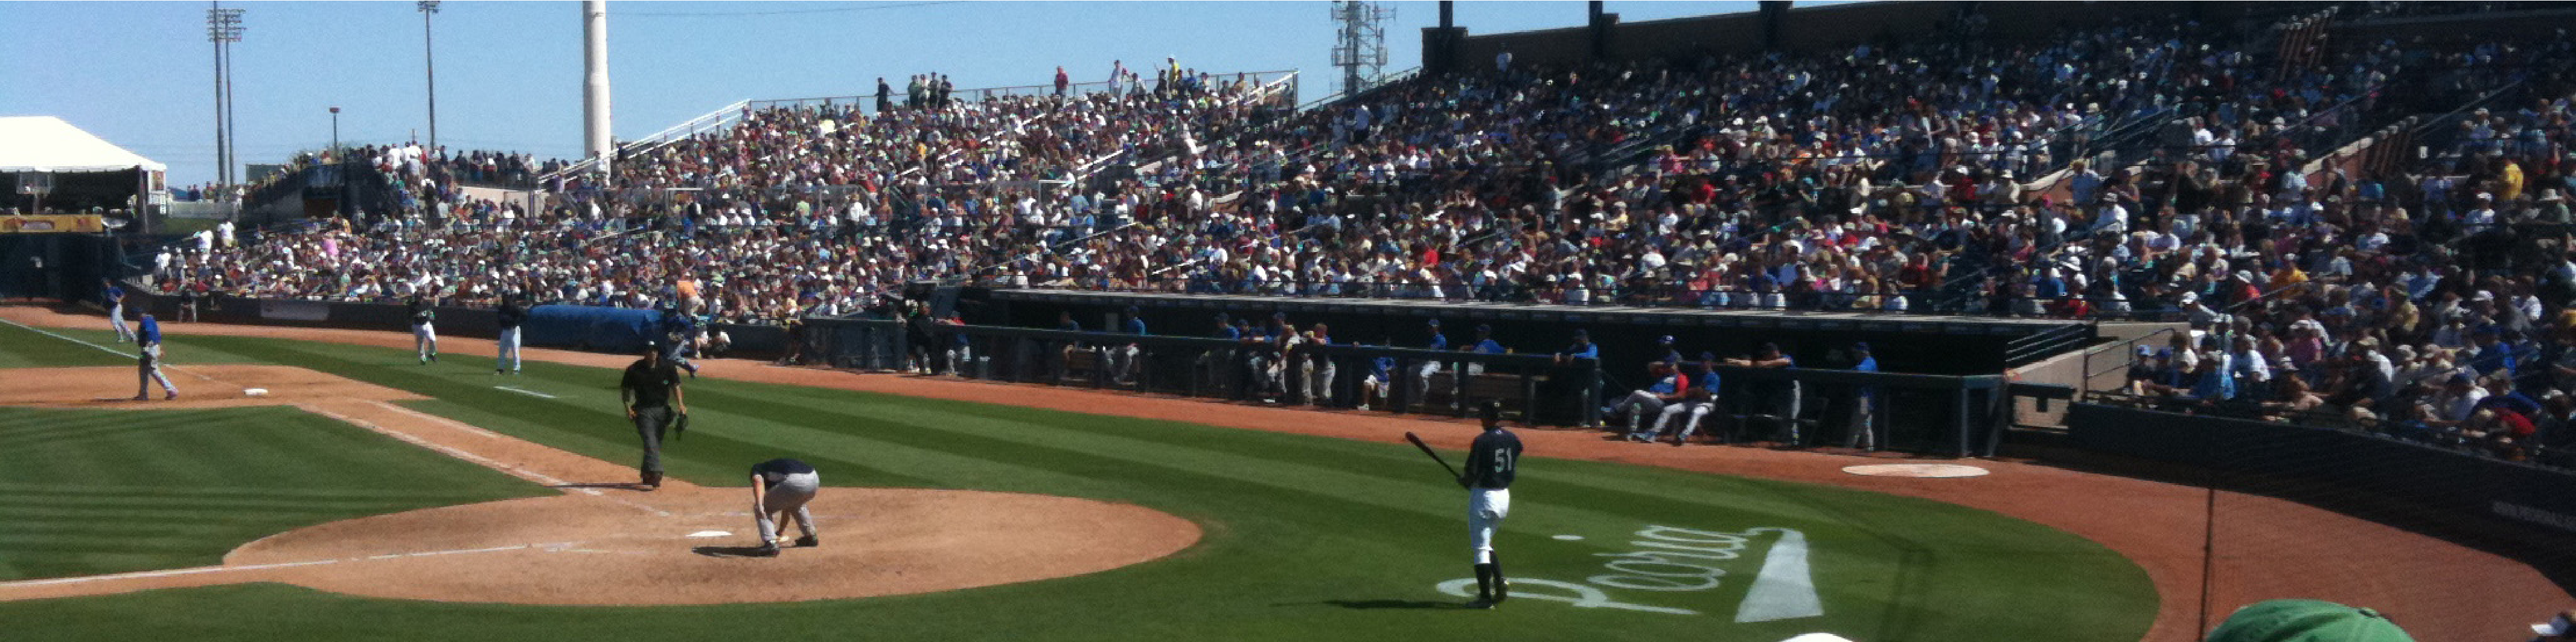
\includegraphics[width=\textwidth]{sampleteaser}
%   \caption{Seattle Mariners at Spring Training, 2010.}
%   \Description{Enjoying the baseball game from the third-base
%   seats. Ichiro Suzuki preparing to bat.}
%   \label{fig:teaser}
% \end{teaserfigure}

%\received{20 February 2007}
%\received[revised]{12 March 2009}
%\received[accepted]{5 June 2009}

%%
%% This command processes the author and affiliation and title
%% information and builds the first part of the formatted document.
\maketitle

\section{Introduction}

Real-time bidding (RTB) in online advertising is fundamentally a problem of stochastic optimal control \cite{RNNControl, RLBid}. 
Advertisers must make sequential bidding decisions to maximize cumulative value, such as gross merchandise value (GMV), while strictly adhering to budget and performance constraints \cite{UnifiedSol}. 
This decision process occurs in a highly volatile market where traffic intensity and competition levels evolve stochastically.
Given the sequential nature of the problem, where current expenditures directly impact future budget availability, reinforcement learning (RL) has emerged as a predominant methodology \cite{RLBid}.
However, deploying RL algorithms directly online is often financially prohibitive due to the high costs of trial-and-error exploration. 
Consequently, a high-fidelity generative world model is indispensable to serve as a surrogate environment for offline policy training and evaluation.
Unfortunately, a critical gap persists: there are currently no usable environment models capable of faithfully reconstructing the market's stochastic dynamics to support downstream Reinforcement Learning.


Despite the architectural advances of generative sequence models in capturing temporal dynamics \cite{Bid2X,DiffBid}, current approaches suffer from fundamental deficiencies when viewed through the lens of stochastic control. 
The primary limitation is their reliance on point prediction objectives that inherently fail to capture the complex marginal properties of auction data. 
Standard approaches typically minimize mean-squared error (MSE) \cite{GAS,GAVE} or perform regression in the logarithmic space \cite{Bid2X,AIGB-Pearl}.
These objectives are statistically ill-posed for RTB data, which is characterized by zero-inflation (a preponderance of zero-valued outcomes arising from lost auctions) and extreme heteroscedasticity (where the variance of feedback scales explosively with the bidding magnitude, leading to orders-of-magnitude differences in noise levels across campaigns).
Specifically, when using MSE on heteroscedastic data, the optimization is dominated by high-variance samples (typically large campaigns), leading to ``gradient dominance'' where the model fails to learn from the majority of smaller samples \cite{kendall2017what}. 
Alternatively, logarithmic regression (Log-MSE) introduces systematic underestimation bias due to Jensen's inequality ($\mathbb{E}[\log Y] \neq \log \mathbb{E}[Y]$). 
Neither approach correctly characterizes the noise structure, yielding a simulator that misrepresents the true market volatility.

Furthermore, point-prediction models fundamentally neglect the joint distribution modeling required for valid control. 
In a bidding context, the agent must navigate the trade-offs between multiple coupled signals (e.g., Cost and GMV). 
However, existing methods typically perform separate regressions for each variable, effectively reducing intrinsically coupled stochastic processes to decoupled deterministic expectations.
This simplification ignores the structural coupling between feedback variables, preventing the simulator from generating realistic coupled trajectories and rendering derived control policies suboptimal in the real, volatile environment.

To address these failures, we propose a physics-informed statistical modeling framework that moves from point regression to full distributional modeling.
Our solution is grounded in the microscopic physical mechanisms of the data generation process.
First, to model the marginal distributions, we axiomatically substantiate that traffic and cumulative value follow Poisson-lognormal and Tweedie-lognormal laws, respectively.
Crucially, we decompose the environmental stochasticity into a hierarchical structure: a latent lognormal intensity field captures the dominant heteroscedasticity (macro-volatility), naturally resolving the gradient dominance issue by explicitly modeling the quadratic scaling of variance with the mean, while the conditional compound Poisson/Tweedie layer handles the mixed discrete-continuous micro-structure (i.e., the accumulation of continuous prices over discrete winning impressions).
Second, to model the dependency structure, we integrate these marginals into a valid joint distribution using a normalizing flow copula.
While standard multivariate models often rely on Gaussian assumptions that imply asymptotic independence, the copula explicitly captures the asymptotic tail dependence arising from the shared winning impressions, ensuring the simulator faithfully reproduces the structural coupling of feedback variables.

In this paper, we establish the rigorous probabilistic foundation for RTB environment modeling. Our contributions are as follows:
\begin{enumerate}
    \item We derive the physical ground truth of feedback dynamics as hierarchical Poisson and compound Poisson-Gamma processes driven by latent lognormal volatility, and propose the zero-inflated generalized beta of the second kind (ZI-GB2) as an efficient operational surrogate.

    \item We address the joint distribution modeling by implementing a normalizing flow copula, which correctly recovers the full dependency structure, including the asymptotic tail dependence inherent in the market.
    
    \item On large-scale real-world production datasets, we show that by correcting the statistical misspecification of prior works, our model achieves state-of-the-art distributional fidelity and exhibits clear neural scaling laws.
\end{enumerate}
This work provides the essential high-fidelity simulator required for future research into constraint-aware stochastic optimal control, ensuring that agents can be trained against the true heavy-tailed and heteroscedastic nature of the auction market.

\section{Problem Formulation}

We formulate the real-time bidding process as a sequential decision-making problem under partial observability. In this section, we define the interaction protocol, the structure of the offline dataset, and formally derive the task of building a generative world model.


\subsection{History-Dependent Decision Process}

The bidding environment is characterized by a latent market state $\mathbf{s}_t$ (e.g., competition intensity, traffic intensity) that is not directly accessible to the advertiser.
Consequently, the decision-making process must rely on the observable history of interactions. 
Formally, we model the bidding task as a history-dependent Markov decision process (HMDP), defined by the tuple $\mathcal{M} = (\mathcal{Y}, \mathcal{A}, \mathcal{H}, P, r, \mathcal{K})$.
Here, the observation space $\mathcal{Y} \subseteq \mathbb{R}^d$ is the set of all possible $d$-dimensional feedback vectors $\mathbf{y}_t$, containing metrics such as costs and conversion counts as detailed in Appendix~\ref{app:seq_view}.
The action space is the set of bidding control vectors $\mathbf{b}_t \in \mathcal{A}$. The precise mathematical definition of $\mathcal{A}$ depends on the specific constrained optimization formulation and is detailed in Appendix~\ref{app:static_view}.
The history space $\mathcal{H}$ constitutes the effective state space representing past interactions. At time $t$, the history is $h_t = (\mathbf{b}_1, \mathbf{y}_1, \dots, \mathbf{b}_{t-1}, \mathbf{y}_{t-1}) \in \mathcal{H}$, where the history space $\mathcal{H}$ is the union of sequences of all lengths, $\mathcal{H} \coloneqq \bigcup_{k=0}^T (\mathcal{A} \times \mathcal{Y})^k$. Here, $(\mathcal{A} \times\mathcal{Y})^0$ represents an empty history.
The transition dynamics $P$ is the probabilistic law governing the environment's response. Given history $h_t$ and action $\mathbf{b}_t$, the environment generates a generalized feedback $\mathbf{y}_t$ according to the conditional joint density $P(\mathbf{y}_t | h_t, \mathbf{b}_t)$.
The immediate reward $r: \mathcal{Y} \to \mathbb{R}$ and the set of performance constraints $\mathcal{K}$ are detailed in Appendix~\ref{app:learn_view}.


\subsection{Offline Dataset and Generative Task}

In the offline RL setting~\cite{levine2020offline}, we learn from a static dataset $\mathcal{D} = \{(\mathbf{c}^{(i)}, \tau^{(i)})\}_{i=1}^L$ of size $L$ collected by a behavior policy, where $\mathbf{c}^{(i)} \in \mathcal{C}$ denotes campaign-specific static covariates (e.g., advertiser type, industry), $\mathbf{\tau}^{(i)} = \{(\mathbf{b}_t, \mathbf{y}_t)\}_{t=1}^{T_i}$ is the sequence of interactions, and $T_i$ is the length of the $i$-th trajectory.

Since the update of history $h_t$ is deterministic once $\mathbf{y}_t$ is observed, the stochasticity of the HMDP is entirely encapsulated in the feedback distribution. Thus, the task of building a generative world model is defined as estimating the conditional joint density:
$
    P_{\theta}(\mathbf{y}_t | h_t, \mathbf{b}_t, \mathbf{c})
$, where $\theta$ is the model parameter.
The challenge addressed in the following sections is that $P_{\theta}$ must respect the specific physical properties of RTB data—namely, zero-inflation, extreme heteroscedasticity, and asymptotic tail dependence—which standard regression objectives fail to capture.

\section{Physics-Informed Statistical Modeling}

The fidelity of a generative world model depends fundamentally on the selection of the conditional distribution family $P_\theta(\mathbf{y}_t | h_t, \mathbf{b}_t)$. While standard statistical model selection practices rely on maximizing likelihood, this data-driven approach encounters a fundamental limitation in the context of RTB.

This section will show that, due to the heavy-tailed nature of auction feedback, statistical criteria alone are insufficient to distinguish between candidate models that imply radically different physical behaviors.
To resolve this ambiguity, we adopt a physics-informed model selection pipeline, deriving the macroscopic statistical laws of RTB—specifically Poisson-lognormal and Tweedie-lognormal—from a set of fundamental axioms describing the microscopic auction process.
Then, we verify these laws through multi-level empirical analysis and operationalize them into a computationally efficient phenomenological surrogate.
Finally, we address the structural coupling between feedback variables. We demonstrate that concurrent feedback metrics exhibit asymptotic tail dependence due to event sharing, which we model using a normalizing flow copula to ensure the model's fidelity in extreme regimes.

\subsection{The Identifiability Crisis in Heavy-Tailed Regimes}

Selecting a marginal distribution family for the feedback vector $\mathbf{y}_t$ is typically framed as a statistical model selection problem. However, our preliminary investigation reveals a critical pathology when applying this logic to RTB data, primarily driven by its extreme heavy-tailedness demonstrated in Appendix~\ref{ssec:heavy_tailedness}.

We evaluated several zero-inflated heavy-tailed candidate distributions on production bidding logs, including skew-lognormal (SLN) \cite{azzalini1985class}, generalized beta of the second kind (GB2) \cite{mcdonald2008some}, gamma lognormal mixture (GLN), Tweedie lognormal mixture (TLN) \cite{tweedie1984index}, lognormal, Burr type XII (BurrXII) \cite{burr1942cumulative}, log-logistic, and gamma.
We observed a ``Flat Minima'' phenomenon: multiple distinct distribution families yielded indistinguishably similar negative log-likelihood (NLL) scores on the test sets. However, as shown in Table~\ref{tab:flat_minima}, their implied physical moments (mean and variance) diverged by orders of magnitude.

% 在正文中插入：
\begin{table}[t]
\centering
\caption{Comparison of goodness-of-fit and moment estimation for predicted GMV (PGMV).}
\label{tab:flat_minima}
% \small
\resizebox{\linewidth}{!}{
\begin{tabular}{lccc}
\toprule
\textbf{Distribution} & \textbf{Test NLL} & \textbf{Mean ($10^3$)} & \textbf{Variance ($10^7$)} \\
\midrule
ZI-SLN         & $9.2484 \pm 0.0394$ & $4.42 \pm 0.08$ & $2.04 \pm 0.13$ \\
ZI-GB2         & $9.2485 \pm 0.0394$ & $4.39 \pm 0.08$ & $2.02 \pm 0.17$ \\
ZI-GLN         & $9.2485 \pm 0.0394$ & $4.37 \pm 0.07$ & $1.90 \pm 0.12$ \\
ZI-GenGamma    & $9.2486 \pm 0.0394$ & $4.36 \pm 0.08$ & $1.51 \pm 0.10$ \\
ZI-TLN         & $9.2491 \pm 0.0397$ & $4.40 \pm 0.09$ & $2.06 \pm 0.13$ \\
ZI-Lognormal   & $9.2495 \pm 0.0391$ & $4.42 \pm 0.07$ & $2.14 \pm 0.10$ \\
ZI-BurrXII     & $9.2546 \pm 0.0393$ & $4.47 \pm 0.08$ & $4.00 \pm 0.93$ \\
ZI-Log-logistic & $9.2569 \pm 0.0390$ & $4.74 \pm 0.08$ & $39.5 \pm 20.9$ \\
ZI-Gamma       & $9.2909 \pm 0.0431$ & $4.38 \pm 0.07$ & $1.28 \pm 0.06$ \\
\bottomrule
\end{tabular}
}
\end{table}

The root of this indeterminacy is because NLL is a point-wise statistic dominated by the bulk of the distribution, a model that minimizes NLL on a finite sample might remains blind to the scarce but influential ``black swan'' events at the tail.
This ambiguity necessitates a shift from purely data-driven model selection to a physics-driven derivation, where the distribution family is identified by the fundamental mechanics of the auction process itself.

\subsection{Physical Generative Mechanism: Axioms, Hypotheses \& Derivations}
\label{ssec:physical_mechanism}
To resolve the identifiability crisis exposed in the previous section, we move beyond curve fitting and reconstruct the data generation process from first principles. We establish a hierarchical theoretical system: starting from fundamental axioms of the auction market, introducing physical hypotheses on system heterogeneity, and deriving the macroscopic distribution forms.

\subsubsection{Fundamental Axioms}
We establish three fundamental axioms based on the intrinsic nature of the advertising business.
These axioms form the first principles for our statistical model.

\begin{axiom}[Discrete Counting]
\label{ax:counting}
Traffic metrics (e.g., PV, Click) are generated by the arrival of discrete users over continuous time. Within a microscopic time window $\Delta t$, this arrival process follows a Poisson point process \cite{kingman1992poisson}. Therefore, the number of winning impressions $N$ within a time step of duration $\Delta t$ follows a Poisson distribution:
\begin{equation}
    N \sim \text{Poisson}(\lambda \Delta t),
\end{equation}
where $\lambda > 0$ represents the instantaneous market intensity.
\end{axiom}

\begin{axiom}[Compound Accumulation]
\label{ax:compound}
Macroscopic feedback metrics $Y$ (e.g., Cost, PGMV) are not directly generated continuous variables; they are the physical summation of discrete microscopic events. That is, $Y = \sum_{i=1}^N X_i$, where $X_i$ is a microscopic mark associated with the $i$-th won impression. In the theory of marked point processes, a mark refers to a random variable (e.g., market price or estimated value) that is attached to each discrete event point \cite{kingman1992poisson}. This formulation defines $Y$ as a compound Poisson process.
\end{axiom}

\begin{axiom}[Shared Event]
\label{ax:shared}
Feedback dimensions associated with the same campaign are coupled through a nested hierarchy of counting processes, reflecting the platform's billing and tracking logic. In a canonical cost-per-click (CPC) based auction system:
\begin{enumerate}
    \item \textbf{Value Coupling:} The cumulative value $V$ (e.g., PGMV) is accumulated over the total winning impressions $N_{PV}$: $V = \sum_{i=1}^{N_{PV}} v_i$, where $v_i$ is the estimated value mark associated with each won impression.
    \item \textbf{Cost Coupling (Poisson Thinning):} The number of clicks $N_{clk}$ is a child process generated via Poisson thinning: $N_{clk} \sim \text{Binomial}(N_{PV}, p_{ctr})$, where $p_{ctr}$ is the click-through rate (CTR). The cumulative cost $C$ is then accumulated over clicks: $C = \sum_{j=1}^{N_{clk}} c_j$, where $c_j$ represents the market price of the $j$-th click.
\end{enumerate}
While $C$ and $V$ are realized over different event counts ($N_{clk}$ and $N_{PV}$ respectively), they remain structurally coupled by the shared latent intensity $\lambda$. 
\textit{Note: While specific hierarchical levels may vary across advertising platforms, e.g., Cost Per Mille (CPM) or optimized CPM (oCPM) models, the principle of shared latent drivers remains a universal physical constraint.}
\end{axiom}



\begin{axiom}[The Dual Nature of Zero-Inflation]
\label{ax:zi_dual}
Zero-valued outcomes in RTB arise from two distinct mechanisms within a hierarchical structure. We define the physical outcome $Y_{phy} = \sum_{i=1}^{N(\lambda)} X_i$.
The total observation $Y$ is the realization of $Y_{phy}$ modulated by a systemic health gate $G$:
\begin{enumerate}
    \item \textbf{Structural Zeros:} Occur when $Y_{phy} = 0$, which is a direct consequence of the counting process where no auctions are won ($N=0$). This occurs with probability $P(Y_{phy}=0|\lambda) = e^{-\lambda\Delta t}$.
    \item \textbf{Anomalous Zeros:} Occur when the systemic health gate fails. We model this gate as a Bernoulli random variable $G \sim \text{Bernoulli}(1-\epsilon)$, where $G=1$ indicates a successful observation channel and $G=0$ indicates a failure (anomalous zero). Here, $\epsilon \in [0, 1]$ represents the latent failure rate.
\end{enumerate}
The final observation is thus defined as the product, $Y = G \cdot Y_{phy}$.
Under this formulation, a zero is ``structural'' if it originates from the Poisson physics ($Y_{phy}=0$) and ``anomalous'' if it originates from the gate failure ($G=0$).
\end{axiom}

\subsubsection{Core Physical Hypotheses}
\label{sssec:hypotheses}

Based on the above axioms, we introduce two key hypotheses describing system heterogeneity. These hypotheses will be empirically verified in Section~\ref{ssec:hypothsis_testing}.

\begin{hypothesis}[Multiplicative Heterogeneity]
\label{hyp:multiplicative}
The market intensity $\lambda$ is governed by the multiplicative interaction of numerous independent factors (e.g., user activity, advertiser competition, and ad attraction). By the central limit theorem in the log-domain, when the number of factors is sufficiently large, the stationary distribution of the intensity field $\lambda$ converges to a log-normal distribution, $\ln \lambda \sim \mathcal{N}(\mu_{L}, \sigma_{L}^2)$.
Physically, this is the macro-volatility of the market where variance scales quadratically with the mean intensity.
\end{hypothesis}

\begin{hypothesis}[Gamma Microscopic Marks]
\label{hyp:gamma_marks}
Individual microscopic marks $X_i$ follow a Gamma distribution: $X_i \sim \text{Gamma}(\alpha, \beta)$.
This choice is motivated by the Tweedie convergence theorem \cite{jorgensen1997theory}, which states that the compound Poisson sum of a wide class of microscopic distributions with positive support and finite moments will asymptotically converge to the compound Poisson-Gamma distribution.
\end{hypothesis}

\subsubsection{Derivation of Model Forms}

Using the axioms and hypotheses, we derive the joint generation mechanism for the environment.


\begin{derivation}[Traffic as Zero-Inflated Poisson-lognormal (ZI-PLN)]
Combining Axiom \ref{ax:counting} and Axiom \ref{ax:zi_dual}, the observed traffic count $N_{obs}$ is the gated realization of the Poisson process: $N_{obs} = G \cdot N_{phy}$. The conditional zero-probability is $P(N_{obs}=0|\lambda) = (1-\epsilon)e^{-\lambda} + \epsilon$. 
Marginalized over the intensity heterogeneity (Hypothesis \ref{hyp:multiplicative}), this defines the zero-inflated Poisson-lognormal distribution, capturing both discrete zero-inflation and extreme heteroscedasticity.
\end{derivation}


\begin{derivation}[Value as Zero-Inflated Tweedie-lognormal (ZI-TLN)]
Combining Axiom~\ref{ax:compound} and Hypothesis~\ref{hyp:gamma_marks}, the generation of microscopic feedback follows a compound Poisson-gamma process.
Consequently, the macroscopic cumulative feedback $Y$ follows a Tweedie distribution with power parameter $1 < p < 2$ \cite{tweedie1984index}, i.e., the compound Poisson-Gamma distribution.
% The mapping from microscopic parameters $(\alpha, \beta, \lambda)$ to macroscopic Tweedie parameters $(\mu, \phi, p)$ is derived as:
% \begin{itemize}
%     \item \textbf{Tweedie Power:} $p = \frac{\alpha+2}{\alpha+1}$, which is determined solely by the shape of the microscopic marks.
%     \item \textbf{Tweedie Mean:} $\mu = \lambda \Delta t \cdot \frac{\alpha}{\beta}$, representing the expected aggregate value.
%     \item \textbf{Dispersion:} $\phi = \frac{(\lambda \Delta t)^{1-p} \cdot \alpha}{\beta^{2-p}(p-1)}$, capturing the scale of fluctuations.
% \end{itemize}
Incorporating the health gate from Axiom \ref{ax:zi_dual}, the observed feedback is $Y_{obs} = G \cdot Y_{phy}$. Its conditional zero-mass is $P(Y_{obs}=0|\lambda\Delta t) = (1-\epsilon)e^{-\lambda\Delta t} + \epsilon$.
When marginalized over the log-normal intensity field $\lambda$ (Hypothesis \ref{hyp:multiplicative}), the final distribution becomes a zero-inflated hierarchical Tweedie-lognormal mixture.
\end{derivation}



\subsection{Empirical Verification of Physical Laws}
\label{ssec:hypothsis_testing}

To verify the hypotheses established in Section~\ref{sssec:hypotheses}, we conduct an empirical analysis on the production data, ensuring that our chosen distribution families are grounded in the verifiable microscopic and macroscopic mechanics of the bidding environment.

\subsubsection{Evidence I: Mark Distribution Verification}
We extracted production bidding instances where the winning impression count (PV) was exactly $1$ with a sample size $N=893$ to analyze the distribution of individual PGMV marks. 
As shown in Table \ref{tab:pgmv_micro_diagnostic}, the Gamma distribution provides an extraordinary fit to the empirical data, yielding an Anderson-Darling (AD) statistic of $3.0465$, which decisively outperforms the Log-normal hypothesis ($AD=18.0661$). This result validates Hypothesis~\ref{hyp:gamma_marks} at the event level, confirming that user value estimates—which lack a hard physical ceiling—naturally follow the skewed, non-Gaussian profile of the Gamma family. Further empirical verification for cost is presented in Appendix~\ref{ssec:cost_gamma_convergence}.


\subsubsection{Evidence II: Latent Posterior Verification}
To provide a direct verification of Hypothesis~\ref{hyp:multiplicative} (Multiplicative Heterogeneity), we inspect the distribution of the latent intensity field in the log-domain.

We numerically inverted the observation model to obtain the posterior samples of the latent variable $\hat{z}_i \sim P(Z\mid Y=y_i)$ for each sample $y_i$, where $Z = \ln \lambda$.
We then inspected the distribution of these inferred latent states against a standard normal distribution.

\begin{table}[htbp]
\centering
\caption{Microscopic distribution for PGMV.}
\label{tab:pgmv_micro_diagnostic}
\begin{tabular}{lcccc}
\toprule
\textbf{Model} & \textbf{NLL} & \textbf{KS Statistic} & \textbf{AD Statistic} \\
\midrule
Log-normal & $3389.17$ & $0.1129$ & $18.0661$ \\
Gumbel & $4358.78$ & $0.2265$ & $95.4868$ \\
\textbf{Gamma} & $\textbf{3293.00}$ & $\textbf{0.0554}$ & $\textbf{3.0465}$ \\
\bottomrule
\end{tabular}
\end{table}

\begin{figure}[h]
    \centering
   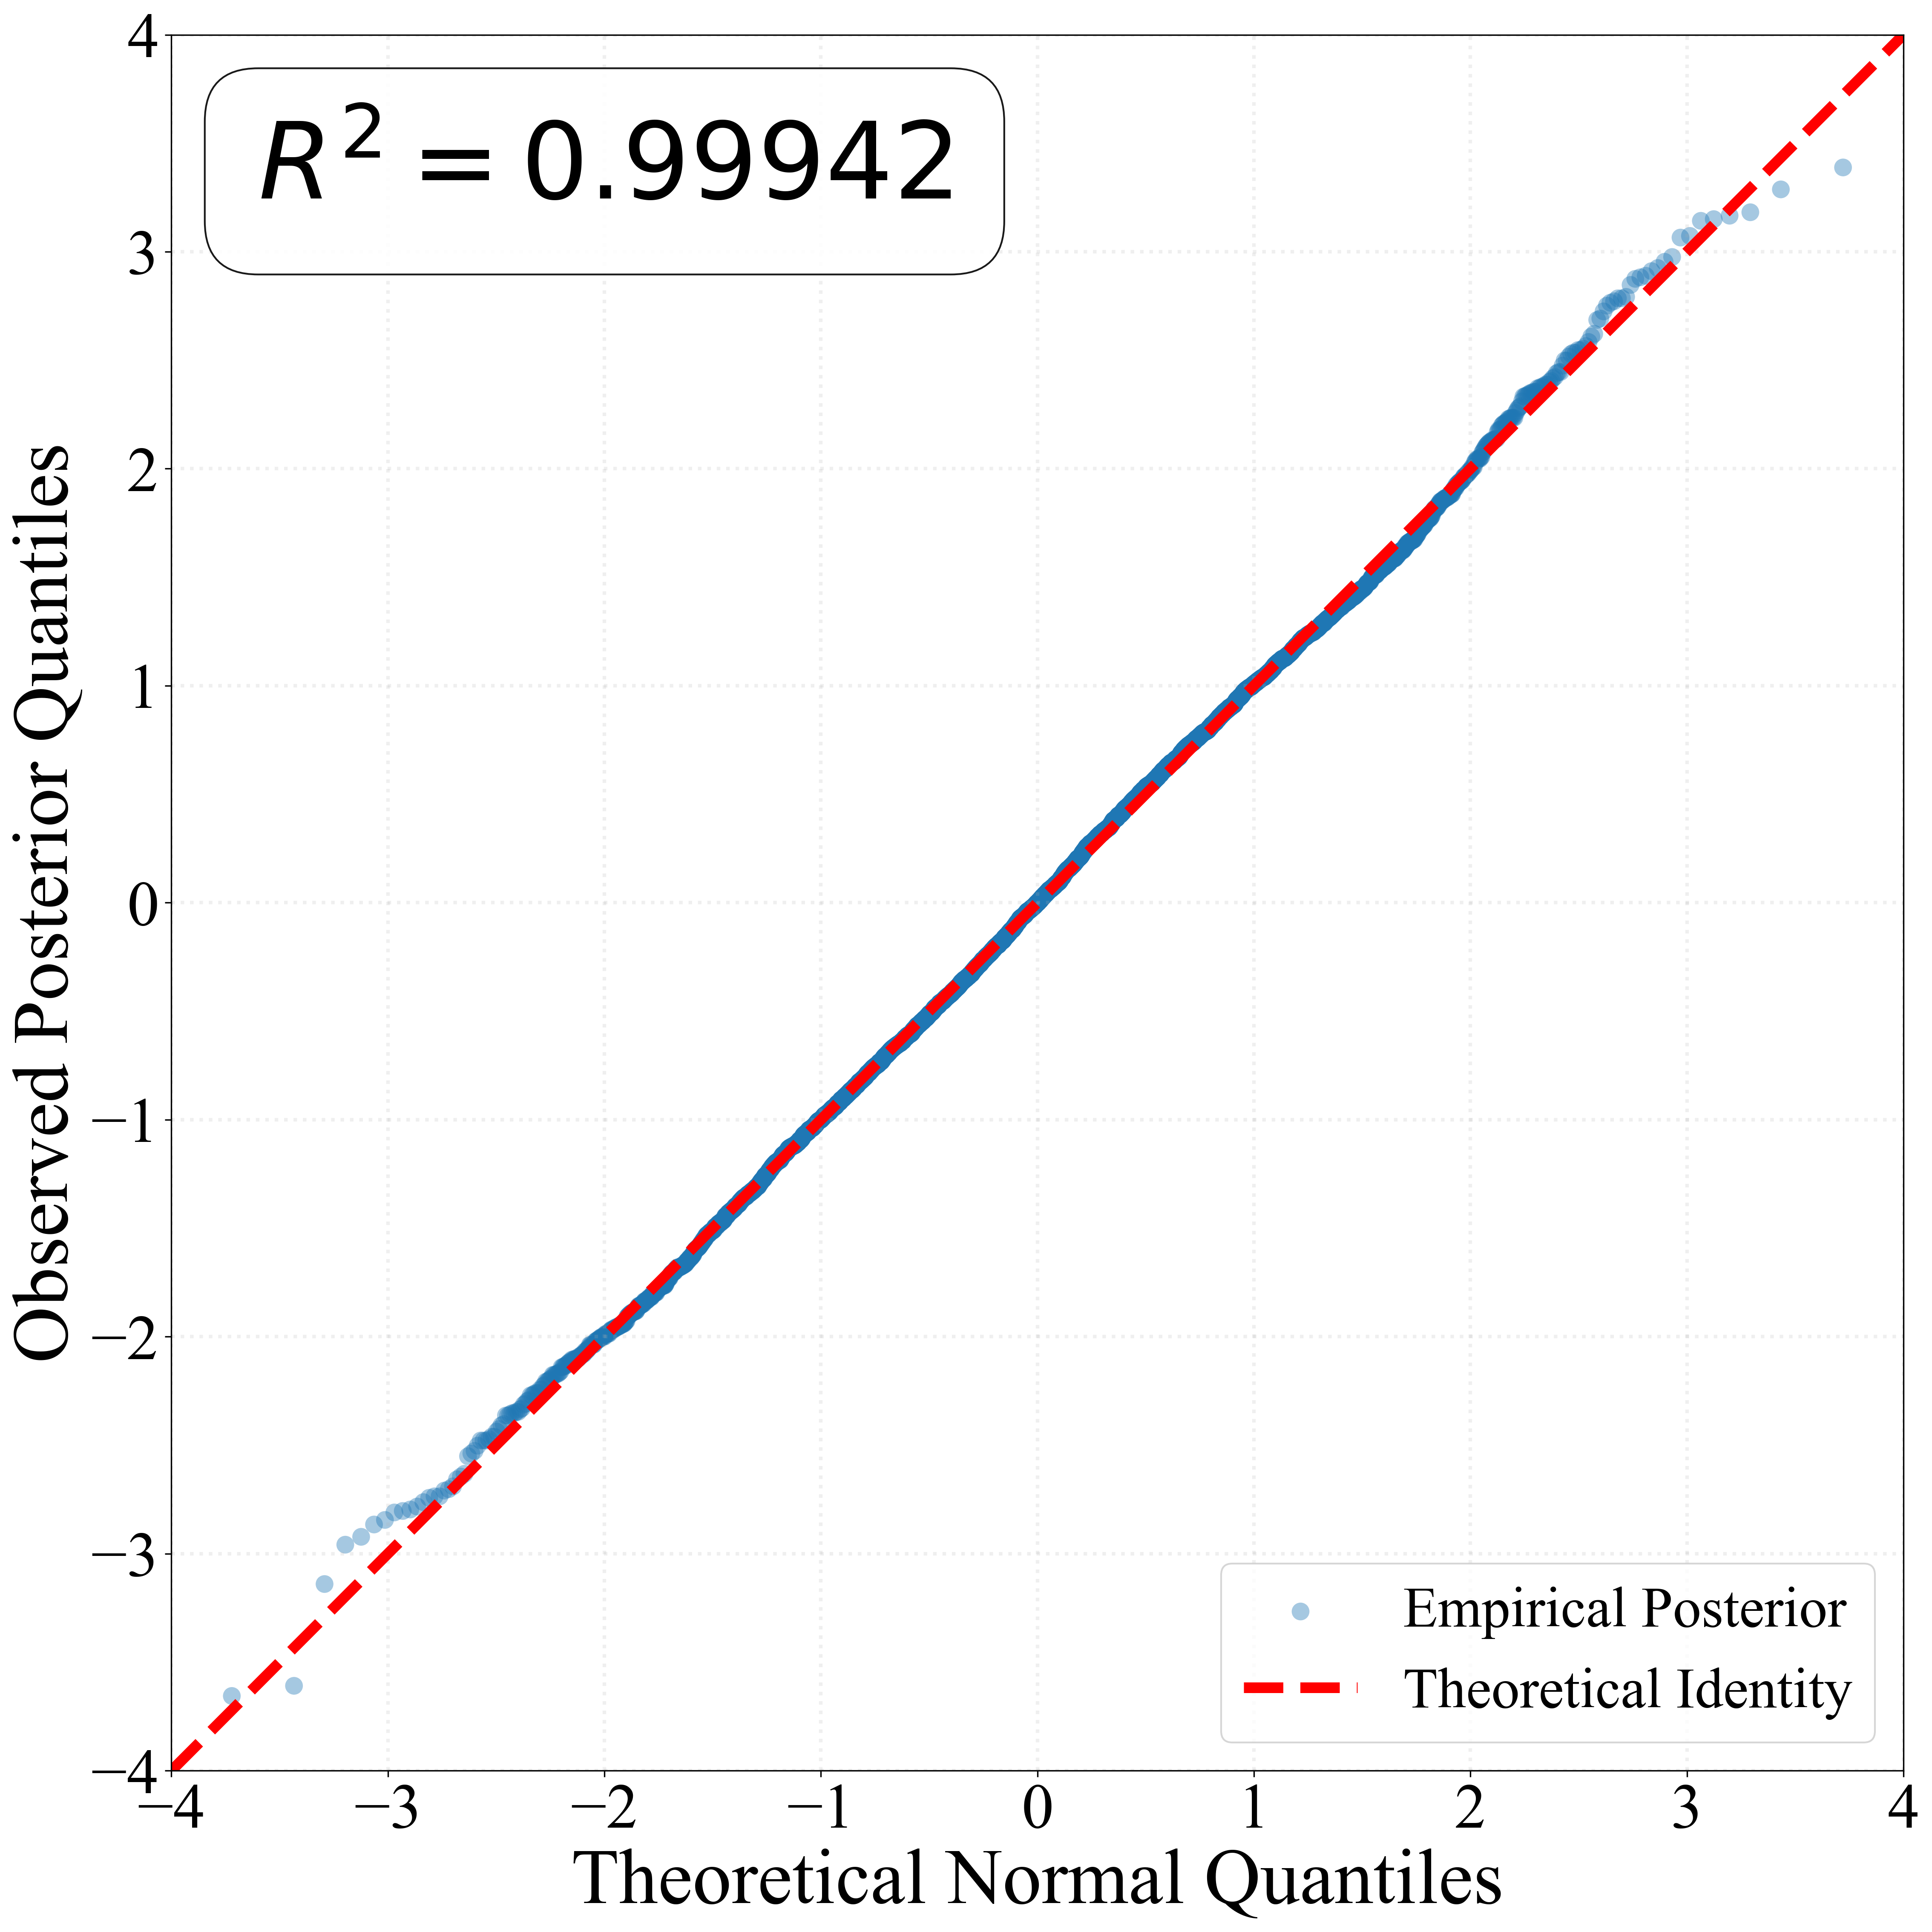
\includegraphics[width=0.7\linewidth]{images/fig3_posterior_qq_plot.png}
    \caption{Q-Q Plot of the inferred latent variable posterior against standard normal.}
    \label{fig:posterior_qq_plot}
\end{figure}

As illustrated in Figure~\ref{fig:posterior_qq_plot}, the data points perfectly align with the $y=x$ line, yielding a linear fit with $R^2 = 0.99942$.
This coefficient of determination indicates that the proposed log-normal model accounts for virtually all the variability in the observed data. 
The extremely high goodness-of-fit rules out alternative hypotheses, such as latent variables following gamma or inverse-Gaussian distributions, providing irrefutable evidence that the macroscopic fluctuations driving RTB dynamics are fundamentally log-normal.

\subsection{Phenomenological Surrogate Selection}
\label{ssec:surrogate_selection}

The above derivation establishes PLN and TLN as the physical ground truth for aggregated bidding feedback.
But, their density lacks a general closed-form expression, typically requiring numerical integration or complex infinite series expansions \cite{dunn2005tweedie} that are computationally prohibitive for the iterative loops of model training and high-frequency RL simulations. In this section, we identify a phenomenological surrogate that is differentiable, computationally efficient, and structurally similar to the physical ground truth.

\subsubsection{Benchmarking Surrogates: The Variance Explosion}
\label{ssec:surrogate_benchmark_main}

To identify the optimal operational surrogate, we conducted a rigorous numerical benchmark across the parameter space of the physical ground truth (Zero-Inflated Tweedie-Lognormal). We evaluated candidate distributions across varying regimes of intensity ($\mu \in \{0.0, 2.0, 4.0, 8.0\}$) and volatility ($\sigma \in [0.4, 2.0]$).

The results, detailed in Appendix~\ref{app:surrogate_experiment}, reveal a critical ``variance explosion'' phenomenon in standard approximations.
As summarized in Table~\ref{tab:surrogate_summary_avg}, standard distributions like ZI-Lognormal and ZI-SLN fail catastrophically to capture the variance, yielding an average variance error (Var Err) exceeding $1000\%$. This occurs because these distributions cannot simultaneously accommodate the heavy zero-mass and the fat tail without pushing their shape parameters into numerically unstable regions.
We also report the error in Value at Risk (VaR), defined as the $\alpha$-quantile of the distribution $F^{-1}(\alpha)$ (here $\alpha=0.99$), to evaluate tail-risk calibration. 

\begin{table}[h]
\centering
\caption{Global average performance across all intensity regimes ($\mu \in \{0, 2, 4, 8\}$).}
\label{tab:surrogate_summary_avg}
\resizebox{0.95\linewidth}{!}{
\begin{tabular}{lcccc}
\toprule
\textbf{Surrogate} & \textbf{NLL Gap} & \textbf{VaR Err} & \textbf{Mean Err} & \textbf{Var Err} \\
\midrule
ZI-Lognormal & $0.0942$ & $54.3\%$ & $41.2\%$ & $1724.6\%$ \\
ZI-SLN & $0.0857$ & $30.5\%$ & $30.6\%$ & $1074.7\%$ \\
\textbf{ZI-GB2 (Ours)} & $\textbf{0.0469}$ & $\textbf{11.5\%}$ & $\textbf{18.3\%}$ & $\textbf{36.6\%}$ \\
\midrule
\textit{ZI-TLN (Oracle)} & $\textit{-0.0009}$ & $\textit{5.9\%}$ & $\textit{4.8\%}$ & $\textit{17.4\%}$ \\
\bottomrule
\end{tabular}
}
\end{table}

In contrast, the proposed ZI-GB2 surrogate demonstrates remarkable structural stability. It reduces the NLL gap significantly and maintains the average variance error within a manageable range ($36.6\%$), closely tracking the physical ground truth (ZI-TLN). This confirms that ZI-GB2 is a strong candidate for capturing macroscopic statistical laws inherent in the auction physics.

\subsubsection{Reparameterized ZI-GB2}

To integrate the ZI-GB2 surrogate into the world model, we implement a reparameterized form that enforces the physical properties derived in Section~\ref{ssec:hypothsis_testing}.
We achieve this by mapping the model's output to a constrained distribution space, ensuring the structural stability of the learned environment.

For a feedback vector $y$, the joint density of ZI-GB2 is:
\begin{equation}
    P(y | \pi, a,b,p,q) = (1 - \pi) \delta(y) + \pi f_{GB2}(y; a, b, p, q),
\end{equation}
where $\delta(y)$ is the Dirac delta at zero, and the Bernoulli gate $\pi$ absorbs both the structural and anomalous zeros. 
The continuous component density of GB2 is:
\begin{equation}
    f_{GB2}(y; a, b, p, q) = \frac{a y^{ap-1}}{b^{ap} B(p, q) [1 + (y/b)^a]^{p+q}},
\end{equation}
where $a > 0$ is the primary shape parameter regulating the power-law decay, $b > 0$ is the scale parameter, and $p, q > 0$ are shape parameters that govern the distribution's behavior in the bulk and the tail, respectively. The term $B(p, q) = \frac{\Gamma(p)\Gamma(q)}{\Gamma(p+q)}$ denotes the Beta function, where $\Gamma(\cdot)$ denotes the Gamma function.

The shape parameter $a$ is vital for tail behavior. We impose a dual-constraint strategy to prevent non-physical moment explosions:
\begin{itemize}
    \item \textbf{Log-Variance Limit:} To prevent latent representation collapse, we bound the variance of the logarithmic, $\text{Var}[\ln X]$. Let $S = \psi'(p) + \psi'(q)$, where $\psi'$ is the trigamma function. We enforce $a \ge a_{\mathrm{min}, 1} = \sqrt{S / \mathcal{V}_{\mathrm{max}}}$, with $\mathcal{V}_{\mathrm{max}} = 1.0$.
    \item \textbf{Finite Skewness Guarantee:} To ensure the existence of the third physical moment, we require $aq > 3$. Thus, $a \ge a_{\mathrm{min}, 2} = 3.0 / q$.
\end{itemize}
The model uses $a = \max(a_{\mathrm{min}, 1}, a_{\mathrm{min}, 2}) + \text{gap}_a$, ensuring the surrogate remains within a physically stable domain throughout training.

\subsection{Modeling Structural Dependencies via Normalizing Flow Copulas}
\label{ssec:joint_modeling}

After establishing the physical laws governing the marginal distributions of bidding feedback, we address the challenge of modeling their joint distribution. In the RTB context, feedback variables (e.g., Cost and GMV) are not independent; they are coupled by the auction mechanism. 
To capture this dependency without constraining the choice of marginals, we adopt the copula framework.

\subsubsection{The Copula Foundation and the Gaussian Fallacy}
Sklar's Theorem \cite{sklar1959fonctions} guarantees that any multivariate joint distribution $F(\mathbf{y})$ can be decomposed into its continuous marginal CDFs $F_i(y_i)$ and a copula function $C: [0, 1]^d \to [0, 1]$ that models the dependency structure among the probability integral transforms $u_i = F_i(y_i)$:
\begin{equation}
    F(\mathbf{y}) = C(F_1(y_1), \dots, F_d(y_d)).
\end{equation}
The joint probability density function is thus factored as:
\begin{equation}
    p(\mathbf{y}) = c(u_1, \dots, u_d) \cdot \prod_{i=1}^d f_i(y_i),
\end{equation}
where $c(\mathbf{u}) = \frac{\partial^d C}{\partial u_1 \dots \partial u_d}$ is the copula density.

A prevalent choice in generative modeling is the Gaussian copula, which assumes latent Gaussian correlations. 
However, we argue that this assumption is fundamentally flawed for auction data due to its inability to model tail dependence. 
The coefficient of upper tail dependence, $\lambda_u$, is defined as the limiting conditional probability that one variable exceeds a high quantile given that another does:
\begin{equation}
    \lambda_u = \lim_{u \to 1^-} P(U_j > u \mid U_i > u).
\end{equation}
For a Gaussian copula with correlation $\rho < 1$, it is theoretically established that $\lambda_u = 0$ \cite{mcneil2015quantitative}, implying asymptotic independence: as events become more extreme, they are assumed to become uncorrelated. This has led to systematic underestimation of correlated defaults during the 2008 financial crisis \cite{li2000default, salmon2009recipe}.


\subsubsection{Physics of Asymptotic Tail Dependence}
In contrast to the Gaussian assumption, RTB dynamics exhibit strong asymptotic tail dependence. Physically, high Cost and high GMV are often simultaneous consequences of a shared underlying driver: a surge in winning impressions (e.g., a ``traffic spike'').
We formalize this intuition in the following proposition:

\begin{restatable}[Existence of Asymptotic Tail Dependence]{proposition}{taildep}
\label{prop:tail_dep}
Under the Axioms and Hypotheses in Section~\ref{ssec:physical_mechanism}, the joint distribution of Cumulative Cost $C$ and Value $V$ exhibits perfect asymptotic tail dependence:
\begin{equation}
    \lambda_u = \lim_{u \to 1^-} P(F_C(C) > u \mid F_V(V) > u) = 1.
\end{equation}
\end{restatable}
\begin{proof}
(Sketch) Both $C$ and $V$ are compound processes summed over the same random number of winning impressions $N$. In the regime of extreme events ($u \to 1^-$), the variance is dominated by the fluctuations of the shared intensity $\lambda$ (the ``traffic volume''). A large deviation in $\lambda$ simultaneously pushes both $C$ and $V$ into their respective tails, locking their co-movement. Detailed proof is provided in Appendix \ref{app:tail_dependence}.
\end{proof}

Proposition \ref{prop:tail_dep} reveals that any generative model relying on Gaussian assumptions will systematically underestimate the joint risk of extreme market events, generating trajectories where high costs and high values essentially decouple in the tail.

\subsubsection{Normalizing Flow Copula}
To capture this non-linear and heavy-tailed dependency, we employ a normalizing flow (NF) copula \cite{wiese2019copula}.
NFs construct complex probability distributions by transforming a simple base distribution (e.g., isotropic Gaussian) through a sequence of invertible, differentiable mappings \cite{kingma2016improved,huang2018neural}.

Let $\mathbf{z} \in \mathbb{R}^d$ be a latent variable drawn from a standard normal distribution $p_Z(\mathbf{z}) = \mathcal{N}(\mathbf{0}, \mathbf{I})$. 
We define a bijection $\mathbf{z} = T_\phi^{-1}(\mathbf{u})$ parameterized by a neural network $\phi$, where $\mathbf{u} \in [0, 1]^d$.
The copula density is given by the change of variables formula:
\begin{equation}
    c_\phi(\mathbf{u}) = p_Z(T_\phi^{-1}(\mathbf{u})) \left| \det \frac{\partial T_\phi^{-1}(\mathbf{u})}{\partial \mathbf{u}} \right|.
\end{equation}
We implement $T_\phi$ using rational quadratic spline flows \cite{durkan2019neural}, which offer high flexibility to learn arbitrary dependency shapes, including the asymmetric tail concentration mandated by Proposition \ref{prop:tail_dep}.

\subsubsection{Empirical Verification}

We validated the necessity of the NF Copula by comparing it against Gaussian, Student-t, and Gumbel copulas on the production dataset. We evaluated both the likelihood fit and the ability to reproduce the physical tail dependence.

\begin{figure}[t]
  \centering
  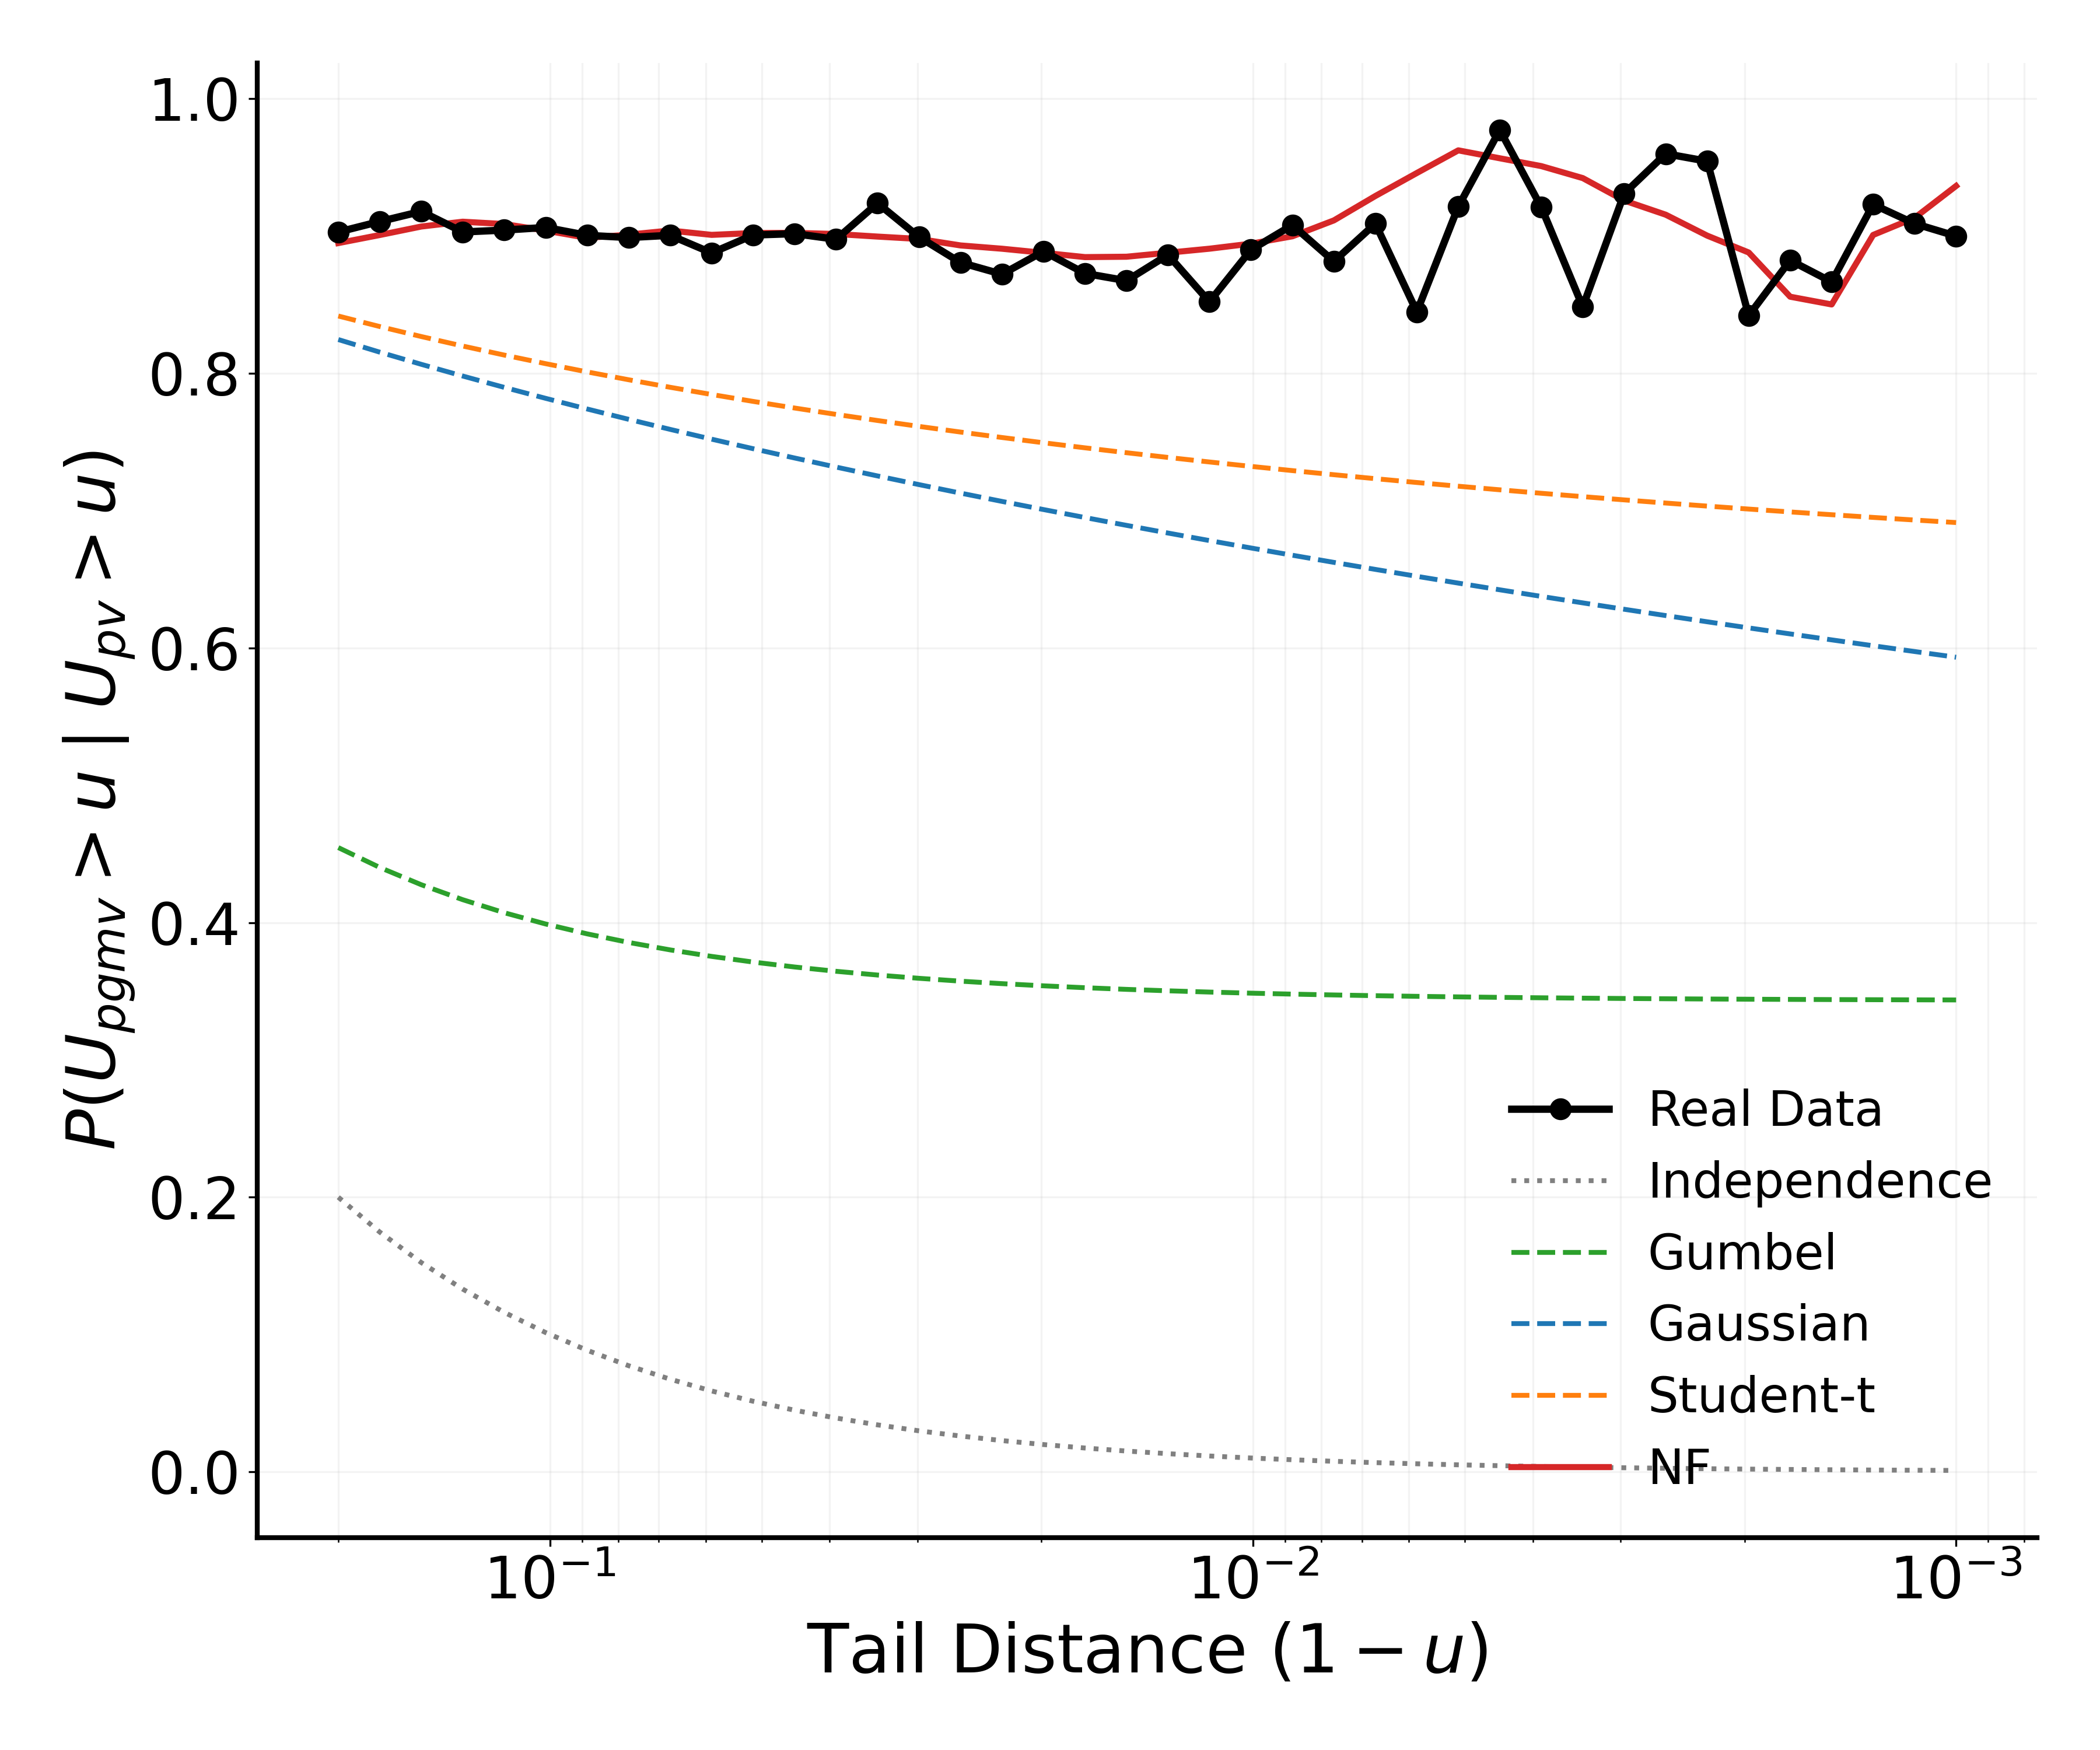
\includegraphics[width=0.8\linewidth]{images/fig4_tail_dependence_cond_prob.png}
  \caption{\textbf{Analysis of asymptotic tail dependence.} The plot shows the conditional probability $P(U_{PGMV} > u \mid U_{PV} > u)$ as a function of the tail distance $(1-u)$. As $u \to 1$, real data maintains high dependence. The normalizing flow correctly captures this trend, whereas the Gaussian copula incorrectly decays toward independence ($\lambda_u=0$).}
  \label{fig:tail_dep_viz}
\end{figure}

\textbf{Likelihood Analysis:} As shown in Table \ref{tab:copula_nll}, the NF Copula achieves the lowest NLL, significantly outperforming the parametric baselines.
The Student-t copula improves upon the Gaussian by allowing $\lambda_u > 0$, but is restricted by its symmetric shape.



\textbf{Tail Dependence Verification:} Figure \ref{fig:tail_dep_viz} visualizes the empirical conditional probability $P(U_{PGMV} > u \mid U_{PV} > u)$ as the threshold $u$ approaches $1$. 
The real data confirms Proposition \ref{prop:tail_dep}: the dependence remains strong and effectively converges to $1$ in the extreme tail.
Crucially, the Gaussian copula exhibits the theoretical ``tail fading'' artifact, dropping towards zero.
Only the normalizing flow successfully models the persistent structural coupling of the market, ensuring that the generated scenarios respect the physics of shared winning events.

\begin{table}[h]
\centering
\caption{Dependence modeling performance}
\label{tab:copula_nll}
\begin{tabular}{lcccc}
\toprule
\textbf{Copula} & Gaussian & Student-t & Gumbel & \textbf{NF} \\
\midrule
\textbf{Test NLL} & $-1.405$ & $-1.441$ & $-0.540$ & $\textbf{-1.909}$ \\
\bottomrule
\end{tabular}
\end{table}

\section{Related Work}

% \subsection{Optimal Bidding and Budget Pacing}
% The theoretical foundations of budget pacing are rooted in constrained optimization and control theory. Early works formulated the problem as a static linear programming (LP) task, establishing that the optimal strategy under stationary market assumptions involves linear bidding with a fixed shadow price \cite{LinBid, UnifiedSol}. To adapt to dynamic environments, feedback control mechanisms, such as Proportional-Integral-Derivative (PID) controllers, were introduced to dynamically adjust the shadow price based on real-time consumption errors \cite{PIDBid}. While these methods provide stability guarantees, they are inherently reactive. They struggle to anticipate non-stationary market shifts (e.g., sudden traffic spikes during holidays) and lack the expressiveness to model the complex, heavy-tailed distribution of market value, often leading to suboptimal pacing in highly volatile environments.

% \subsection{Generative AI for Auto-bidding}
% To capture the non-stationarity of RTB environments, the field has increasingly pivoted towards data-driven sequence modeling. Early attempts utilized Recurrent Neural Networks (RNNs) to learn temporal dependencies in winning prices and click-through rates \cite{RNNControl}. With the advent of Generative AI, recent approaches have adopted more sophisticated architectures. For instance, Conditional Diffusion Models have been employed to generate optimal trajectory distributions \cite{DiffBid}, while Transformer-based methods \cite{GAS, GAVE, AIGB-Pearl} leverage attention mechanisms to model bidding policies and value functions over long horizons.

% However, these "black-box" generative models suffer from a critical limitation we term \textbf{Confounded Learning}. They typically model the joint distribution of historical states and actions, failing to distinguish between the \textit{exogenous} dynamics of the market and the \textit{endogenous} bias of historical bidding policies. Consequently, they risk learning spurious correlations—such as attributing low costs to high bids simply because bids were historically raised during low-traffic periods—which fundamentally violates the causal monotonicity required for reliable counterfactual reasoning.

% \subsection{Bidding Foundation Models}
% The concept of a "Foundation Model" for bidding has recently emerged to address the heterogeneity of advertising scenarios. Bid2X \cite{Bid2X} represents the state-of-the-art in this direction, employing a unified Transformer architecture to encode diverse bidding data (e.g., different ad formats and objectives). It notably introduces a zero-inflated projection layer to handle data sparsity.

% Despite its success in representation learning, Bid2X exhibits significant \textbf{Statistical Failures}. To manage multi-scale data, it performs regression in the logarithmic domain. Due to Jensen's inequality ($\mathbb{E}[\log Y] \neq \log \mathbb{E}[Y]$), this introduces a systematic underestimation bias when mapped back to the linear space where budget constraints operate. Furthermore, it focuses on fitting conditional means rather than the full probability distribution. In a highly fluctuating environment characterized by heavy-tailed Tweedie-like noise, mean-fitting is statistically inefficient and insufficient for robust control. Our work addresses this by grounding the foundation model in rigorous statistical laws (Zero-Inflated Tweedie and Copulas) and physical causal structures.

Our research sits at the confluence of generative sequence learning, auction mechanism analysis, and statistical physics.
% In this section, we critically review the evolution of these fields through a hierarchical lens: starting from the generative sequence modeling paradigms that tackle sequential decision and simulation tasks, descending to the microscopic landscape forecasting of individual auction outcomes.
% We then identify the missing physical link: the statistical physics of sparse compound processes that aggregates micro-events into macro-responses, and finally address the structural tail dependence governing the coupling of multidimensional feedback.

% Across these domains, we highlight a persistent methodological gap: the failure of standard regression techniques to capture the heavy-tailed volatility and structural coherence inherent to the auction mechanism.


\subsection{Generative Sequence Modeling in RTB}
Recent research has extensively leveraged generative sequence architectures—ranging from recurrent neural networks (RNNs) \cite{elman1990finding} to Transformers \cite{vaswani2017attention} and Diffusion models \cite{ho2020denoising}—to tackle the sequential decision-making challenges in RTB. 
We categorize these advancements into two parallel tracks: policy optimization and environment simulation.

On the policy optimization track, the focus lies on generating optimal bidding trajectories.
Early works parameterized bidding policies via RNNs \cite{RNNControl}. 
The paradigm subsequently shifted towards Transformer-based decision making, where methods like GAS \cite{GAS} and GAVE \cite{GAVE} adapt Decision Transformers \cite{chen2021decision}, modeling the dependencies between target returns and action sequences.
More recently, generative planning has emerged, with DiffBid \cite{DiffBid} and AIGB-Pearl \cite{AIGB-Pearl} leveraging conditional diffusion models or model-based planners to generate high-value cost trajectories.

On the environment simulation track, the goal is to model the market's feedback dynamics. Bid2X \cite{Bid2X}, representing the current state-of-the-art, introduces architectural innovations by fusing iTransformer encoders \cite{liu2024itransformer} with Transformer decoders to model bid-response trajectories. 

However, across both tracks, we argue that the field has witnessed \textit{architectural progress} but \textit{statistical stagnation}.
While these methods utilize advanced backbones to capture temporal correlations, they fundamentally rely on point-prediction paradigms (e.g., MSE or Log-MSE) designed for homoscedastic signals.
By treating volatile financial feedback merely as generic time-series tokens, they fail to capture the statistical properties of RTB data.

\subsection{Deep Landscape Forecasting}
Another significant strand of research focuses on Deep Landscape Forecasting (DLF), which aims to predict the probability distribution of the market price for individual auctions \cite{RLBid, DLF, ou2023deep}. 
These methods typically employ survival analysis to handle the censorship inherent in second-price auctions, devising specialized loss functions to learn the winning probability at the impression level \cite{li2022arbitrary}.
While these models are grounded in the mechanics of single auctions, they predominantly characterize the microscopic and often static price landscape.
They do not explicitly model how these micro-outcomes aggregate into the macroscopic, dynamic bidding responses (e.g., total Cost and GMV over a decision step) that are subject to the agent's time-varying budget constraints.
Our work bridges this gap by deriving the macroscopic distribution laws directly from these microscopic mechanisms.


\subsection{Statistical Physics of Compound Processes}
Accurate simulation of RTB feedback requires traversing the scale from discrete micro-events to continuous macro-outcomes.
Statistically, this aggregation is described by compound processes, where random magnitudes accumulate over a random count.
The Tweedie family, formalized in statistical dispersion theory \cite{jorgensen1997theory}, provides a unified framework for such processes.
It theoretically grounds the variance-to-mean power laws ($Var(\mu) \propto \mu^p$) empirically observed in ecology (Taylor's Law) \cite{taylor1961aggregation} and has effectively become the standard for modeling aggregate claims in actuarial science \cite{smyth2002fitting}.
Extensions like zero-inflated Tweedie (ZIT) \cite{ZIT} further address excess sparsity distinct from stochastic zeros.

Despite their foundational status, the application of these compound distributions remains largely absent in the RTB literature, where sparsity is often treated via ad-hoc heuristics rather than derived likelihoods \cite{Bid2X}.
From the perspective of statistical physics, the efficacy of these models stems from a universality principle: the Tweedie convergence theorem \cite{jorgensen1997theory}.
This theorem establishes that for any exponential dispersion model, the variance function asymptotically follows a power law $V(\mu) \sim \mu^p$ under scaling operations, effectively singling out the Compound Poisson-Gamma distribution ($1 < p < 2$) as the unique domain of attraction for mixed discrete-continuous distributions with probability mass at zero.
Distinct from ``physics-informed'' methods that embed continuous PDEs \cite{raissi2019physics}, our work embeds this discrete event microstructure.

\subsection{Multivariate Tail Dependence Modeling}
Copula theory, grounded in Sklar's theorem, enables separate modeling of marginal distributions and their dependence structure \cite{joe2014dependence}. It is particularly valuable for heavy-tailed data where standard normalizing flows fail because Lipschitz-bounded transformations cannot faithfully map heavy tails to Gaussian latent spaces \cite{jaini2020tails}. To address this, several copula-based deep architectures have been proposed.
CM flows disentangle marginal from joint learning \cite{wiese2019copula}. \cite{laszkiewicz2021copulabased} integrate the copula structure into the base distribution of flow-based models. COMET Flows target multivariate extremes and tail dependence \cite{COMETFlows}. Deep Archimedean copulas parameterize copula generators with neural networks \cite{ling2020deep}, while mTAF modulate tail behavior via adaptive base distributions \cite{laszkiewicz2022marginal}. These methods collectively advance the modeling of multivariate heavy-tailed distributions \cite{resnick2007heavy}, but have not been applied to RTB environments.
The normalizing flow copula adopted in this paper is an application of CM flows to mixed continuous-discrete marginals.


\begin{table*}[htbp]
\centering
\caption{Performance comparison.}
\label{tab:perf_sub1_256}
\begin{tabular}{lcccccccc}
\toprule
Method & \multicolumn{2}{c}{CLICK} & \multicolumn{2}{c}{COST} & \multicolumn{2}{c}{PV} & \multicolumn{2}{c}{VALUE} \\
\cmidrule(lr){2-3} \cmidrule(lr){4-5} \cmidrule(lr){6-7} \cmidrule(lr){8-9}
 & SMAPE & CRPS & SMAPE & CRPS & SMAPE & CRPS & SMAPE & CRPS \\
\midrule
BFM (ZI-GB2) & $0.685$ & $0.688$ & $0.775$ & $0.605$ & $0.479$ & $12.127$ & $0.738$ & $3.434$ \\
BFM (MSE) & $1.763$ & $1.417$ & $1.680$ & $0.860$ & $1.974$ & $50.462$ & $1.756$ & $8.231$ \\
BFM (ZI-SLN) & $0.664$ & $0.671$ & $0.777$ & $0.607$ & $0.473$ & $14.483$ & $0.752$ & $3.553$ \\
Informer (ZI-GB2) & $0.352$ & $0.638$ & $0.269$ & $\textbf{0.316}$ & $\textbf{0.314}$ & $\textbf{8.810}$ & $\textbf{0.342}$ & $\textbf{2.091}$ \\
Informer (MSE) & $1.226$ & $0.473$ & $1.358$ & $0.660$ & $0.388$ & $14.803$ & $0.567$ & $3.670$ \\
Informer (ZI-SLN) & $\textbf{0.188}$ & $\textbf{0.381}$ & $\textbf{0.266}$ & $0.330$ & $0.377$ & $14.200$ & $0.348$ & $2.586$ \\
NST (ZI-GB2) & $0.709$ & $0.729$ & $0.775$ & $0.609$ & $0.486$ & $13.547$ & $0.739$ & $3.501$ \\
NST (MSE) & $1.435$ & $0.958$ & $1.640$ & $0.799$ & $0.483$ & $17.123$ & $0.818$ & $4.700$ \\
NST (ZI-SLN) & $0.667$ & $0.677$ & $0.777$ & $0.612$ & $0.490$ & $16.317$ & $0.750$ & $3.642$ \\
Transformer (ZI-GB2) & $0.706$ & $0.734$ & $0.772$ & $0.603$ & $0.471$ & $12.155$ & $0.733$ & $3.445$ \\
Transformer (MSE) & $1.432$ & $0.944$ & $1.635$ & $0.787$ & $0.476$ & $16.663$ & $0.808$ & $4.606$ \\
Transformer (ZI-SLN) & $0.669$ & $0.688$ & $0.776$ & $0.606$ & $0.474$ & $15.118$ & $0.745$ & $3.585$ \\
\bottomrule
\end{tabular}
\end{table*}

\section{Experiments}
\label{sec:experiments}

This section empirically validates our physics-informed generative world model framework. 
Our evaluation focuses on two core hypotheses: 
(1) \textbf{Distributional Fidelity:} Whether the physically derived ZI-GB2 objective recovers the stochastic dynamics of the bidding environment better than standard regression baselines; 
(2) \textbf{Scalability:} Whether the physics-informed formulation exhibits favorable neural scaling laws compared to deterministic approaches.

\subsection{Experimental Setup}

\subsubsection{Datasets}
We used a large-scale collection of industrial bidding logs from the Taobao advertising platform. Following the protocol in Bid2X~\cite{Bid2X}, we evaluated our models in large datasets that span diverse advertiser constraints and durations of campaigns.

\subsubsection{Baselines and Architectures}
To disentangle the contribution of the model architecture from the statistical modeling objective, we evaluate four distinct backbone networks combined with three different loss functions. The backbones include Transformer~\cite{vaswani2017attention}, Non-Stationary Transformer (NST)~\cite{liu2022nonstationary}, Informer~\cite{zhou2021informer}, and Bid2X~\cite{Bid2X}.
For each backbone, we compare three objectives, including Log-MSE, ZI-SLN NLL, and ZI-GB2 NLL.

\subsubsection{Evaluation Metrics}
Given the heavy-tailed nature of the feedback (e.g., GMV), standard metrics like RMSE are dominated by outliers. We adopt two robust metrics to evaluate both point estimation accuracy and distributional calibration:

\textbf{1. Symmetric Mean Absolute Percentage Error (SMAPE):} 
A relative error metric robust to scale variations, defined as:
\begin{equation}
    \text{SMAPE} = \frac{1}{N} \sum_{i=1}^N \frac{|y_i - \hat{y}_i|}{(|y_i| + |\hat{y}_i|)/2},
\end{equation}
where $\hat{y}_i$ is the predicted expectation.

\textbf{2. Continuous Ranked Probability Score (CRPS):}
A strictly proper scoring rule that measures the compatibility of the predicted cumulative distribution function $F$ with the observation $y$:
\begin{equation}
    \text{CRPS}(F, y) = \int_{-\infty}^{\infty} (F(z) - \mathbb{1}\{y \le z\})^2 dz,
\end{equation}
where $F$ is the CDF of the prediction distribution.
CRPS generalizes the absolute error to probabilistic forecasts. The expectation of CRPS is zero if and only if the prediction distribution equals the true data distribution.
Additional metrics are reported in Appendix~\ref{app:add_exp}.
\subsection{Performance on Distributional Fidelity}

Table~\ref{tab:perf_sub1_256} summarizes the performance of all architecture-objective pairs. The empirical results reveal three critical insights into the modeling of auction dynamics:

\textbf{1. The Failure of Deterministic Objectives.}
Across all backbone architectures (BFM, Informer, NST, Transformer), the standard MSE objective consistently yields the poorest performance.
For instance, in the Informer architecture, switching from MSE to our physics-informed ZI-GB2 objective reduces the PV CRPS from $14.803$ to $8.810$ and the Value CRPS from $3.670$ to $2.091$.
This huge disparity confirms our core premise: deterministic point-prediction objectives are statistically ill-posed for the heavy-tailed, heteroscedastic nature of RTB feedback.

\textbf{2. The ``Hidden'' Variance Explosion.}
A critical observation regarding the ZI-SLN baseline is its apparent stability.
In Section~\ref{ssec:surrogate_benchmark_main}, we predicted a variance explosion for lognormal families.
However, in the large-scale experiments, ZI-SLN did not diverge.
This stability is artificial: to prevent numerical collapse during training, we imposed a hard constraint on the shape parameter ($\sigma \le 1.0$).
Post-training analysis reveals that the learned $\sigma$ for ZI-SLN consistently hits this upper bound ($\sigma \approx 1.0$), indicating that the model is struggling to express the true data variance but is mechanically clamped.
In contrast, ZI-GB2 naturally fits the data variance without hitting parameter boundaries, offering a mathematically consistent solution rather than an engineered fix.

\textbf{3. Generalizability across Architectures.}
Our physics-informed loss function demonstrates consistent improvements independent of the encoder architecture.
Notably, the Informer + ZI-GB2 combination achieves the state-of-the-art performance across almost all metrics (highlighted in bold), surpassing the BFM (Bid2X) baseline.
This suggests that while advanced attention mechanisms (like those in Bid2X or Informer) are important for temporal feature extraction, the statistical alignment of the training objective with the physical generation process is the dominant factor in determining the fidelity of the world model.

\subsection{Neural Scaling Laws}

To verify whether our physics-informed formulation can effectively leverage increasing computational resources, we investigate the scaling behavior of the model performance with respect to the parameter size $M$. We train the Bid2X backbone with varying capacities using three objectives.

As illustrated in Figure~\ref{fig:scaling_law}, we observed a power-law relationship between the test loss $L$ and the number of model parameters $M$,
\begin{equation}
    L(M) \propto M^{-\alpha}.
\end{equation}
Crucially, the scaling exponent $\alpha$ for the ZI-GB2 model ($\alpha_{GB2} \approx 0.16$) is significantly larger than that of the MSE baseline ($\alpha_{MSE} \approx 0.12$). 
This implies that the physics-informed model is more sample-efficient and gains greater performance improvements from scale. 
This confirms that respecting the physical laws of the data generation process is a prerequisite for unlocking the full potential of large foundation models in computational advertising.

\begin{figure}[htbp]
  \centering
  % Placeholder for the scaling law plot
  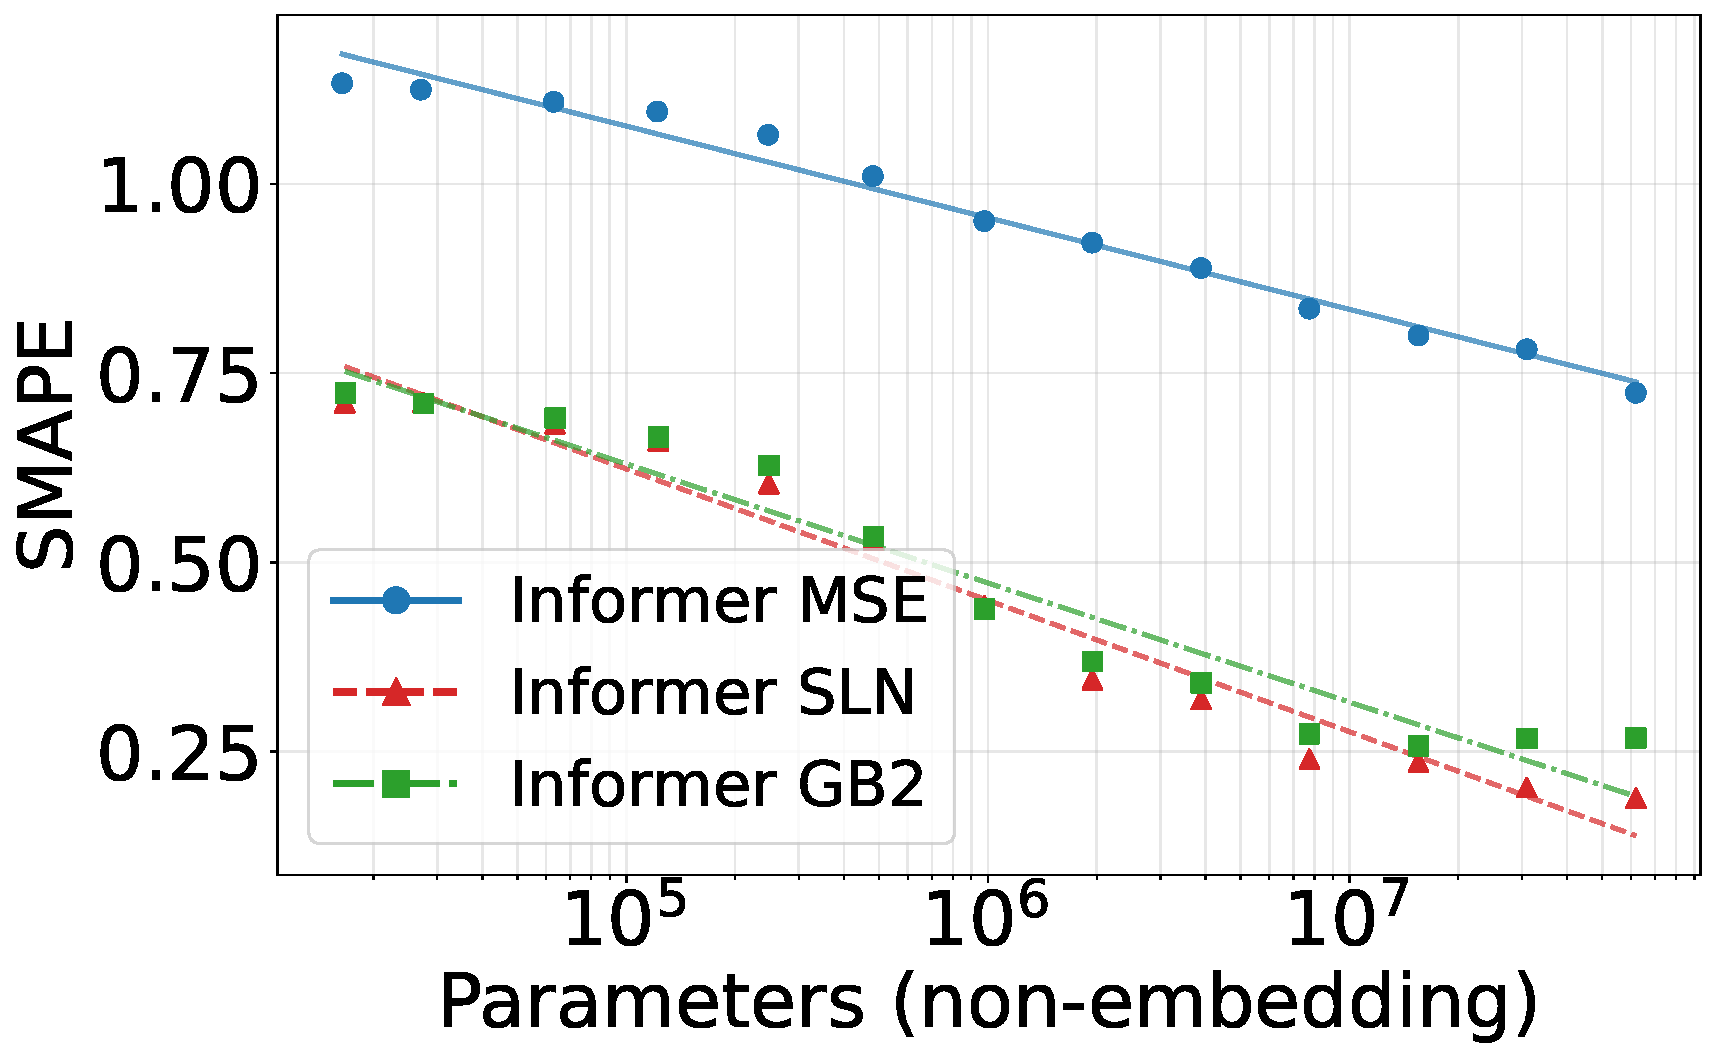
\includegraphics[width=0.8\linewidth]{images/fig5_median-smape_vs_params.pdf}
  \caption{\textbf{Neural Scaling Laws.} The test CRPS on the Crowd dataset as a function of model parameters. The physics-informed  model (ZI-GB2) exhibits a steeper scaling slope compared to the deterministic baseline (MSE), indicating superior data efficiency and potential for scaling.}
  \label{fig:scaling_law}
\end{figure}

\section{Conclusion and Future Outlook}

This work revisits the fundamental epistemology of environment modeling in computational advertising.
We demonstrate that the prevailing bottleneck in RTB simulation is not architectural capacity, but statistical identification.
By abandoning the convenient but flawed assumptions of homoscedasticity and Gaussianity, and instead deriving the generative laws from the microscopic physics of auction mechanics, we have established that the stochasticity of the market is structurally heavy-tailed and coupled.

However, our operationalization of these physical laws remains an approximation. While the proposed ZI-GB2 surrogate effectively mitigates the variance explosion problem found in standard lognormal baselines, it acts merely as a phenomenological proxy.
Empirically, it does not strictly converge to the theoretical Oracle (ZI-TLN) in all regimes, nor does it achieve absolute dominance over the ZI-SLN baseline.
Finding a closed-form, differentiable density that offers a tighter bound to the exact compound Poisson-gamma likelihood remains an open mathematical challenge.

Furthermore, our derivation relies on the multiplicative heterogeneity hypothesis, assuming that market intensity follows a lognormal distribution.
While this captures the general volatility, real-world advertising environments likely exhibit more extreme heterogeneity governed by power laws in the far tail (e.g., power-law distributions of advertiser budgets or Pareto-distributed traffic spikes due to marketing events).
Future work will extend our framework to model these ``super-heavy-tailed'' phenomena, thereby pushing the boundary of simulation fidelity in highly non-stationary environments.

% In this paper, we have presented a physics-informed generative world model for Real-Time Bidding, grounding the statistical modeling of auction feedback in the microscopic axioms of compound processes. By deriving the Zero-Inflated Tweedie-Lognormal (ZI-TLN) law as the physical ground truth and introducing the Normalizing Flow Copula, we addressed the fundamental deficiencies of deterministic objectives in capturing the heteroscedasticity and tail dependence of market dynamics.

% By traversing the scale from microscopic axioms to macroscopic laws, we proved that the feedback dynamics are governed by hierarchical compound Poisson-Gamma processes driven by lognormal volatility.
% We operationalized this physical ground truth into the Zero-Inflated Generalized Beta of the Second Kind (ZI-GB2) surrogate, which naturally resolves the gradient dominance issue in heavy-tailed regimes.
% Furthermore, we addressed the structural coupling of multidimensional feedback through a Normalizing Flow Copula, theoretically and empirically validating that high-cost and high-value events exhibit perfect asymptotic tail dependence—a phenomenon missed by Gaussian assumptions.

% Empirical results on large-scale production datasets demonstrate that correcting these statistical priors enables the model to achieve state-of-the-art distributional fidelity.
% Crucially, our physics-informed formulation exhibits clearer neural scaling laws compared to standard regression baselines, suggesting that statistical alignment with the data generation process is a prerequisite for scaling up bidding foundation models.
% This work provides the essential high-fidelity environment required for future research into safe, constraint-aware stochastic optimal control, ensuring that offline policies are robust to the true volatility of the market.

%%
%% The acknowledgments section is defined using the "acks" environment
%% (and NOT an unnumbered section). This ensures the proper
%% identification of the section in the article metadata, and the
%% consistent spelling of the heading.
\begin{acks}
To Robert, for the bagels and explaining CMYK and color spaces.
\end{acks}

%%
%% The next two lines define the bibliography style to be used, and
%% the bibliography file.
\bibliographystyle{ACM-Reference-Format}
\bibliography{sample-base}


%%
%% If your work has an appendix, this is the place to put it.

\newpage

\appendix


\section{Complete Formulation of Constrained Bidding and Optimization Objectives}
\label{app:constrained_formulation}

This appendix provides the detailed mathematical background for the constrained bidding problem discussed in this paper.
We first present the optimal bidding function derived from a static optimization perspective. 
Next, we describe how this function is integrated into our sequential decision-making framework, where the agent dynamically controls its parameters.
Finally, we introduce two formalizations for trajectory-level constrained optimization.

\subsection{Static View: Primal LP and the USCB Bidding Function}
\label{app:static_view}

We adopt the theoretical foundation of the Unified Solution to Constrained Bidding (USCB) \cite{UnifiedSol}.
In a static setting with $N$ candidate auctions, the advertiser seeks to maximize total value subject to a budget constraint $B$ and $M$ performance constraints.
The primal problem is formulated as a linear program (LP):
\begin{equation}
\begin{aligned}
    \max_{\mathbf{x}} \quad & \sum_{i=1}^N x_i v_i \\
    \text{s.t.} \quad & \sum_{i=1}^N x_i c_i \le B \\
    & \frac{\sum_{i=1}^N \mathbb{c}_{ij} x_i}{\sum_{i=1}^N \mathbb{p}_{ij} x_i} \le \mathbb{k}_j, \quad \forall j \in [M] \\
    & 0 \le x_i \le 1, \quad \forall i,
\end{aligned}
\end{equation}
where $[M]\coloneqq\{1,\ldots,M\}$, $v_i$ and $c_i$ are the value and market price of impression $i$.
For each KPI constraint $j$, $\mathbb{c}_{ij} = c_i \mathbb{I}_{CR_j} + \mathbb{q}_{ij} (1 - \mathbb{I}_{CR_j})$, where $\mathbb{I}_{CR_j}$ is the indicator for cost-related constraints, i.e., constraints that restricts the unit cost of certain advertising event, such as cost per action and cost per click. For non-cost-related constraints, $\mathbb{q}_{ij}$ represents a performance indicator that acts as the ``cost'' signal for NCR constraints.
For instance, in a CTR constraint, $\mathbb{q}_{ij}$ might be set to $1$ to count impressions in the numerator, while $\mathbb{p}_{ij}$ represents the click probability.

As proved in \cite{UnifiedSol}, the optimal bid $b_i^*$ is derived from the dual problem via complementary slackness. For any impression $i$, the optimal bidding function is given by Equation (2) in \cite{UnifiedSol}:
\begin{equation}
\label{eq:uscb_formula_appendix}
    b_{i}^{*}=w_{0}^{*}v_{i}-\sum_{j \in \mathcal{K}}w_{j}^{*}(\mathbb{q}_{ij}(1-\mathbb{I}_{CR_{j}})-\mathbb{k}_{j}\mathbb{p}_{ij}),
\end{equation}
where $w_{0}^{*}>0$ and $w_{j}^{*}\ge0$ are the optimal dual variables (shadow prices) that reflect resource scarcity and constraint pressure.

\subsection{Sequential View: From Static LP to Dynamic Parameter Control}
\label{app:seq_view}
The static theory provided in \cite{UnifiedSol} prescribes the functional form of the optimal bid price, but it assumes the existence of optimal parameters $\vec{w}^*$ calculated over a complete, known dataset. In the dynamic RTB environment defined in Section 2, future impressions arrive sequentially and are unknown. To bridge this, we transform the problem into a sequential control task where the RL agent acts as a dynamic solver of the dual variables.

At each time step $t$, the policy $\pi(\mathbf{b}_t | h_t)$ maps the interaction history to an action vector $\mathbf{b}_t \equiv [w_{0,t}, w_{1,t}, \dots, w_{M,t}]^\top \in \mathcal{A}$. Physically, this action constitutes the agent's real-time estimation of the optimal shadow prices required to navigate the remaining budget and constraint surplus. Once the agent outputs $\mathbf{b}_t$, it is held constant for the duration of the time step. Every sequentially arriving impression $i$ within the interval $[t, t+1)$ is bid upon using the linear formula in Eq. (\ref{eq:uscb_formula_appendix}), substituting the agent's chosen action $\mathbf{b}_t$ for the weights. 

To bridge micro-decisions to macro-observations, we define the microscopic outcome vector $\mathbf{u}_i \in \mathbb{R}^d$, where $d=2M+2$, for each auction $i$ as a vector containing all potential feedback signals:
\begin{equation}
    \mathbf{u}_i \coloneqq [v_i, c_i, \mathbb{c}_{i1}, 、\mathbb{p}_{i1}, \dots, \mathbb{c}_{iM}, \mathbb{p}_{iM}]^\top.
\end{equation}
The macroscopic feedback $\mathbf{y}_t \in \mathcal{Y} \subseteq \mathbb{R}^d$ observed at the end of step $t$ is the physical summation of these realized outcomes:
\begin{equation}
    \mathbf{y}_t \coloneqq \sum_{i \in \Delta_t} x_i \mathbf{u}_i.
\end{equation}
Under this formulation, the world model $P(\mathbf{y}_t | h_t, \mathbf{b}_t)$ is essentially learning the macroscopic physics of how a high-frequency auction market aggregates thousands of micro-decisions governed by shadow prices $\mathbf{b}_t$.

\subsection{Learning View: Trajectory-Level Optimization Objectives}
\label{app:learn_view}

The advertiser's objective is to learn a target policy $\pi$ that maximizes the expected total impression values subject to $M$ global performance constraints.
We define the set of constraints $\mathcal{K}$ and the optimization objectives through projection mappings $g_v, g_c^k, g_p^k: \mathcal{Y} \to \mathbb{R}_{\ge 0}$ that extract specific dimensions from the aggregated feedback $\mathbf{y}_t$:
\begin{equation}
    v_t = g_v(\mathbf{y}_t), \quad \mathbb{c}_{t,k} = g_c^k(\mathbf{y}_t), \quad \mathbb{p}_{t,k} = g_p^k(\mathbf{y}_t).
\end{equation}
For example, $g_c^k(\mathbf{y}_t) = \mathbf{e}_{2k+1}^\top \mathbf{y}_t$, where $\mathbf{e}_{2k+1}$ is the basis vector corresponding to the index of $c_{ik}$ in $\mathbf{u}_i$.
Let $R_{\Sigma}=\sum_{t=1}^T g_v(\mathbf{y}_t)$ be the total impression value. Let $C_{\Sigma, k}(\tau) = \sum_{t=1}^T g_c^k(\mathbf{y}_t)$ and $P_{\Sigma, k}(\tau) = \sum_{t=1}^T g_p^k(\mathbf{y}_t)$ denote the cumulative cost and performance signals associated with the $k$-th constraint. We consider two distinct constraint formulations for this problem.

\paragraph{Formulation 1: Ratio of Expectations (RoE).}
The standard approach aligns strictly with the business definition of global constraints. It formulates the problem as a constrained optimization on the risk-neutral ratio of expectations:
\begin{equation}
\label{eq:optimization_target_roe_app}
    \max_{\pi} \quad J(\pi) = \mathbb{E}_{\tau \sim \pi} \left[ R_{\Sigma} \right] \quad \text{s.t.} \quad \forall k \in \mathcal{K}, \quad \frac{\mathbb{E}_{\tau \sim \pi}[C_{\Sigma, k}]}{\mathbb{E}_{\tau \sim \pi}[P_{\Sigma, k}]} \le \Gamma_k.
\end{equation}
This problem is typically solved via the Lagrangian method, introducing dual variables $\lambda_k$ to optimize the saddle point of the Lagrangian. This formulation aims for the exact satisfaction of the mean constraint but is sensitive to the variance of the constraint surplus $S_k = C_{\Sigma, k} - \Gamma_k P_{\Sigma, k}$ during the gradient estimation.

\paragraph{Formulation 2: Soft Constraint.}
Alternatively, we may consider a robust formulation, induced by \cite{auction_net}, that internalizes constraints into a multiplicative soft penalty. This approach transforms the constrained optimization into an unconstrained utility maximization problem:
\begin{equation}
\label{eq:optimization_target_soft_app}
    \max_{\pi} \quad J_{\mathrm{soft}}(\pi) = \mathbb{E}_{\tau \sim \pi} \left[ R_{\Sigma} \cdot \prod_{k \in \mathcal{K}} \Psi\left( \frac{C_{\Sigma, k}}{P_{\Sigma, k}}, \Gamma_k; \beta_k \right) \right],
\end{equation}
where the penalty function $\Psi(z, \Gamma; \beta)$ adopts a generalized power-law truncation form:
\begin{equation}
    \Psi(z, \Gamma; \beta) = \min\left(1, \left(\frac{\Gamma}{z + \epsilon}\right)^{\beta}\right).
\end{equation}
Here, $\beta_k > 0$ controls the risk sensitivity, and $\epsilon>0$ exists to avoid division by zero. This formulation effectively saturates the penalty for extreme violations, bounding the influence of outliers on the policy gradient and enhancing robustness in heavy-tailed market environments.

\section{Additional Empirical Verification}
\subsection{Empirical Evidence of Heavy Tails}
\label{ssec:heavy_tailedness}
We begin by diagnosing the tail behavior of key feedback metrics using the Hill estimator, a standard non-parametric tool for identifying the tail index $\alpha$ of a power-law distribution.
As shown in Figure \ref{fig:heavy_tail_evidence}, while the estimated tail index $\alpha$ for metrics such as Predicted GMV (PGMV) and cost remains above the theoretical infinite-variance boundary ($\alpha=2$), the relatively low values confirm the presence of a heavy tail where extreme fluctuations carry disproportionately high probability mass compared to exponential families.
This physical property poses a significant challenge: in finite samples, the rarest but most influential tail events are sparsely represented, making the likelihood surface extremely flat and insensitive to the specific tail structure of the chosen distribution.

\begin{figure}[htbp]
  \centering
   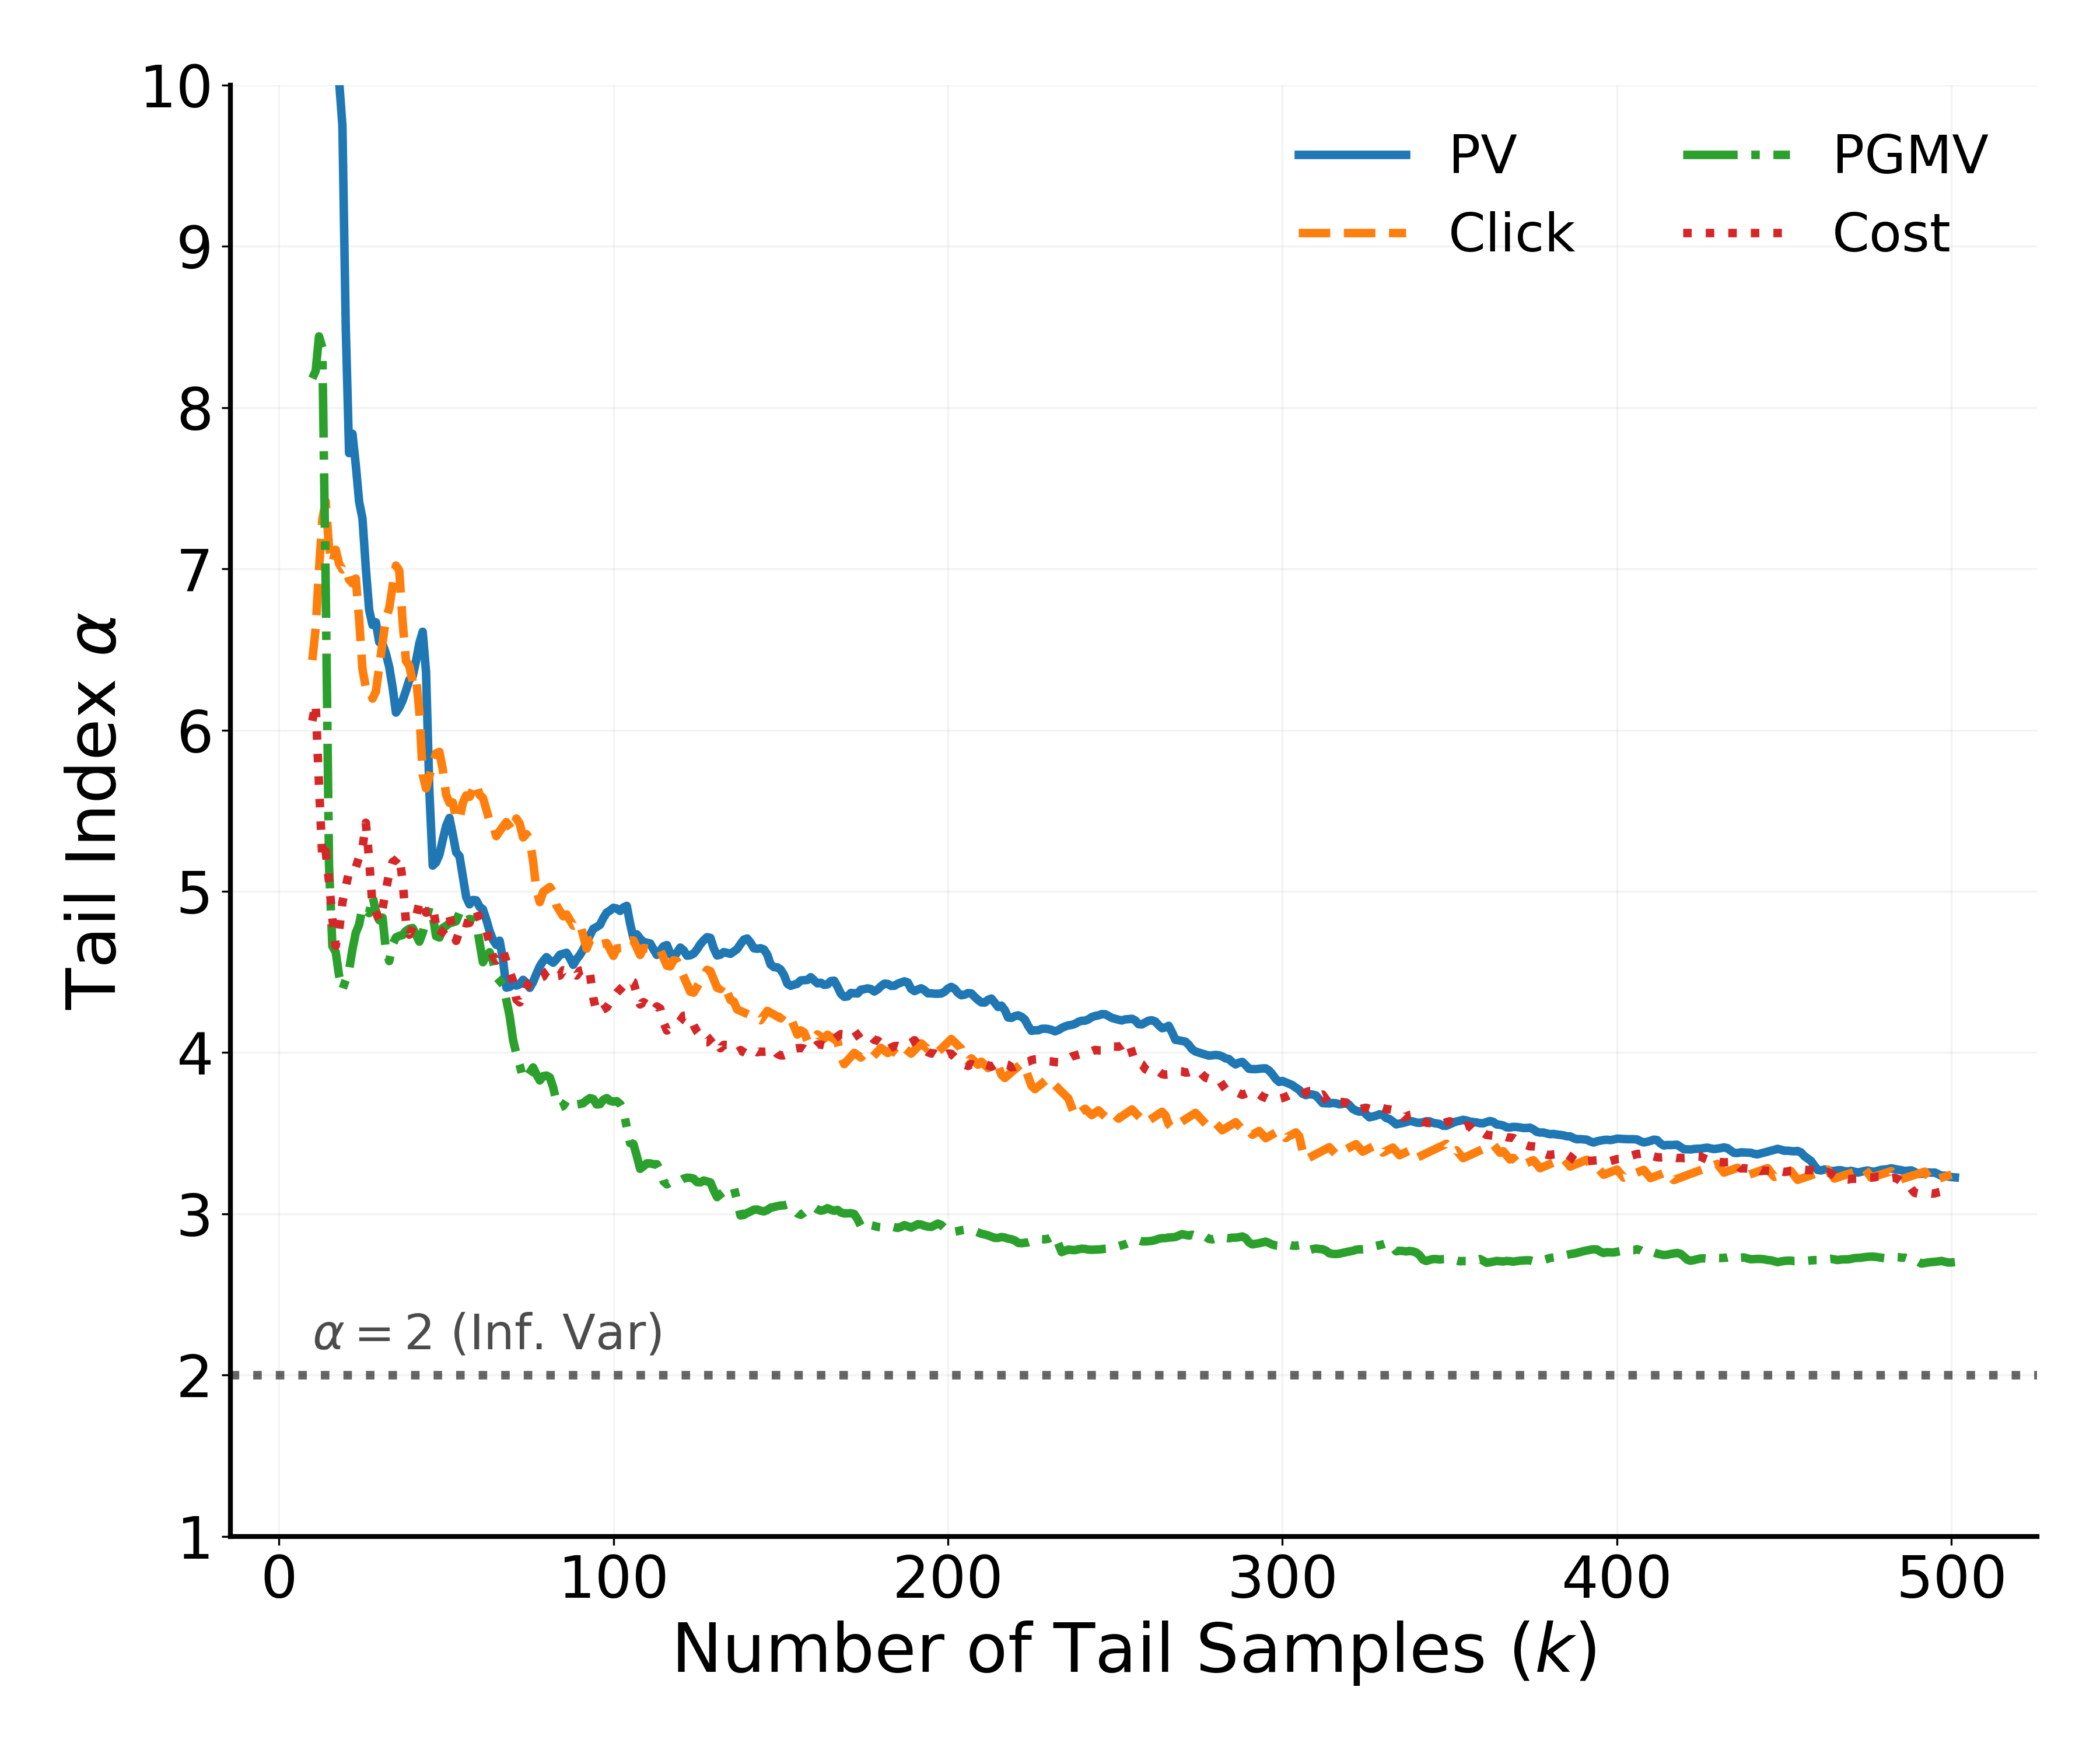
\includegraphics[width=0.8\linewidth]{images/fig1_heavy_tail_viz.png}
  \caption{Quantitative verification of heavy-tailedness. The Hill plot demonstrates that the tail index $\alpha$ stabilizes at values far lower than those required for Gaussian behavior. The persistence of this plateau across a large number of tail samples indicates that extreme market events are a structural feature of the environment, not stochastic outliers.}
  \label{fig:heavy_tail_evidence}
  \vspace{-0.3cm}
\end{figure}

\begin{table}[htbp]
\centering
\caption{Microscopic distribution for cost.}
\label{tab:cost_micro_diagnostic}
\begin{tabular}{lcccc}
\toprule
\textbf{Model} & \textbf{NLL} & \textbf{KS Stat} & \textbf{AD Stat} \\
\midrule
\textbf{Beta} & $715.44$ & $\textbf{0.0453}$ & $\textbf{3.7536}$ \\
Truncated Normal & $\textbf{713.17}$ & $0.0592$ & $14.5383$ \\
Gumbel & $792.77$ & $0.0464$ & $4.4918$ \\
Gamma & $834.86$ & $0.1049$ & $19.3738$\\
Log-normal & $1053.55$ & $0.1561$ & $52.3260$ \\
\bottomrule
\end{tabular}
\end{table}

\subsection{The Microscopic Distribution of Cost}
\label{ssec:cost_gamma_convergence}

A distinct phenomenon emerges when analyzing the cost of a single click ($N=944$). As illustrated in Table \ref{tab:cost_micro_diagnostic}, the cost distribution is best described by bounded distributions such as the Beta distribution ($AD=3.7536$), whereas both Gamma and Log-normal perform poorly. 
This indicates that unlike latent value estimations, transaction costs are subject to systemic truncation, inducing a compact support.


To justify the use of Gamma marks despite this micro-level divergence, we conducted an analytic convergence analysis. We matched the first two moments of a Beta mark $X_{B}$ and a Gamma mark $X_{G}$ and computed the statistical distance between their respective Compound Poisson aggregates $Y = \sum_{i=1}^\lambda X_i$ as a function of intensity $\lambda$. 
As illustrated in Figure~\ref{fig:convergence}, our numerical results show that both the Kullback–Leibler (KL) divergence and the $1$-Wasserstein distance normalized by the standard deviation $\sigma$ drops dramatically with the increase of the Poisson intensity.
This rapid decay is dictated by the Tweedie convergence theorem \cite{jorgensen1997theory} and provide irrefutable evidence for the structural stability of the Tweedie attractor: the micro-level structure is rapidly erased by aggregation, and Gamma serves as the canonical representative of the universality class.

\begin{figure}[htbp]
    \centering
    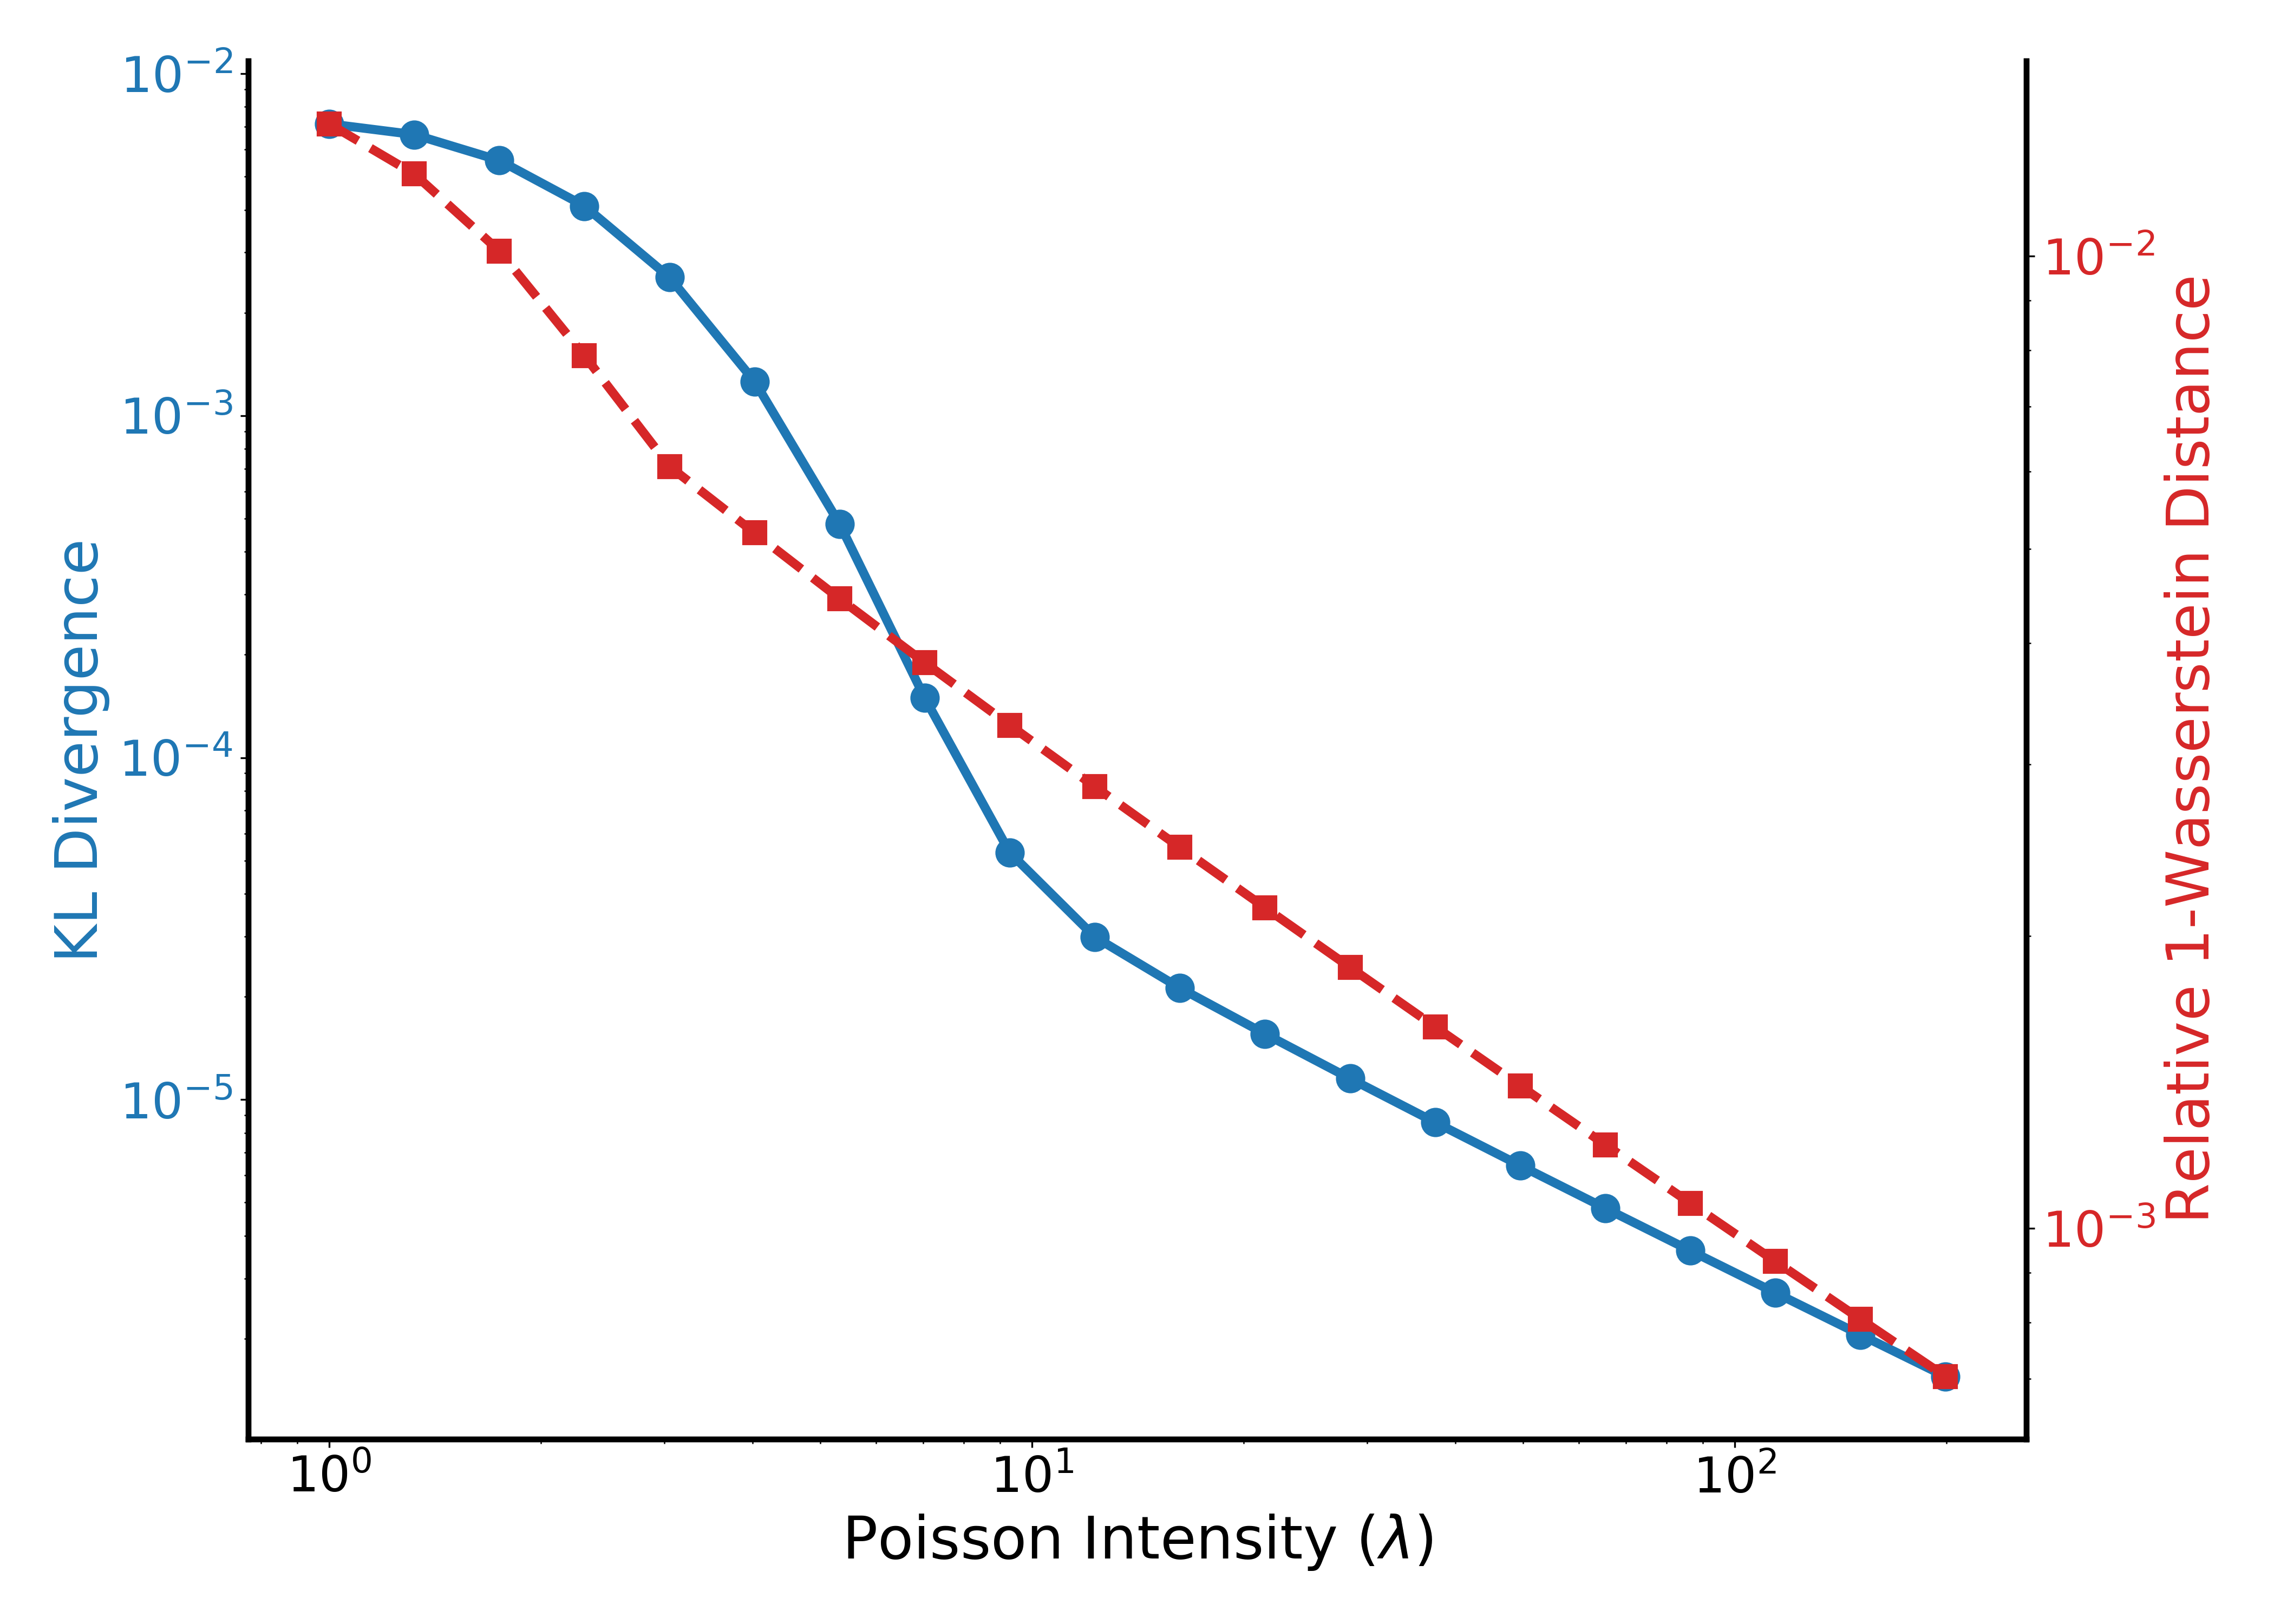
\includegraphics[width=0.9\linewidth]{images/fig2_tweedie_lambda_convergence.png}
    \caption{Convergence from compound Poisson-beta to Tweedie. The logarithmic axes show the rapid decay of KL divergence and relative $1$-Wasserstein distance as intensity $\lambda$ increases, confirming the attractor properties of the Gamma-Tweedie system.}
    \label{fig:convergence}
\end{figure}


\section{Surrogate Selection Experiments}
\label{app:surrogate_experiment}

In this section, we provide the complete experimental setup and detailed results for the phenomenological surrogate selection process discussed in Section~\ref{ssec:surrogate_benchmark_main}. The goal is to identify a distribution family that is computationally efficient (closed-form density) yet statistically indistinguishable from the physical ground truth (Tweedie-Lognormal).

\subsection{Experimental Setup}

\paragraph{The Physical Manifold}
We define the ground truth data generation process using ZI-TLN distribution derived in Section~\ref{ssec:physical_mechanism}. We sweep the hyper-parameter space to cover diverse market conditions:
\begin{enumerate}
    \item \textbf{Intensity Scale ($\mu \in \{0.0, 2.0, 4.0, 8.0\}$):} Mean levels, representing campaigns ranging from extremely sparse regimes to high-volume environments.
    \item \textbf{The Tweedie Power Index ($p \in [1.1, 1.9]$):} Controlling the microscopic mark's shape by $p \coloneqq \frac{\alpha+2}{\alpha+1}$. Notably, since the TLN family collapses to the PLN law when $p=1$, the experiments for traffic metrics (counts) are implicitly covered within this unified framework, eliminating the need for a separate benchmark for discrete outcomes.
    \item \textbf{Latent Volatility ($\sigma \in [0.4, 2.0]$):} Capturing the macroscopic multiplicative heterogeneity of market intensity.
\end{enumerate}

\paragraph{Robust Fitting Strategy}
To avoid local minima during MLE, we implemented a coarse-to-fine dynamic optimization pipeline. 
For each point on the $(\mu, p, \sigma)$ grid:
\begin{enumerate}
    \item \textbf{Initialization:} We utilize a stochastic dynamic k-nearest neighbor approach, seeding the optimizer with parameters from the best-performing neighbors in the grid to ensure continuity on the accuracy surface.
    \item \textbf{Optimization:} We employ the L-BFGS algorithm with strong Wolfe line search and multiple random restarts to strictly minimize the NLL.
    \item \textbf{Evaluation:} We compute robust metrics using numerical integration on a high-resolution grid with $2^{12}$ points to ensure the ground truth statistics, such as mean, variance, P99 VaR (99\% value at risk), are exact.
\end{enumerate}


\subsection{Detailed Results}

\begin{table*}[htp]
\centering
\caption{Detailed performance metrics.}
\label{tab:surrogate}
\begin{tabular}{clcccc}
\toprule
\textbf{Intensity} & \textbf{Model} & \textbf{NLL Gap} & \textbf{VaR Err ($\%$)} & \textbf{Mean Err ($\%$)} & \textbf{Var Err ($\%$)} \\
\midrule
\multirow{4}{*}{\shortstack{$\mu=0.0$\\(Sparse)}} 
& ZI-Lognormal & $0.2546$ & $109.7$ & $104.2$ & $3355.5$ \\
& ZI-SLN & $0.2460$ & $75.0$ & $85.9$ & $2722.9$ \\
& \textbf{ZI-GB2} & $\textbf{0.1643}$ & $\textbf{23.6}$ & $\textbf{55.3}$ & $\textbf{44.3}$ \\
& \textit{ZI-TLN} & $\textit{-0.0009}$ & $\textit{6.3}$ & $\textit{5.7}$ & $\textit{21.6}$ \\
\midrule
\multirow{4}{*}{\shortstack{$\mu=2.0$\\(Medium)}} 
& ZI-Lognormal & $0.1032$ & $81.4$ & $42.6$ & $3295.4$ \\
& ZI-SLN & $0.0841$ & $32.9$ & $21.1$ & $1466.3$ \\
& \textbf{ZI-GB2} & $\textbf{0.0216}$ & $\textbf{9.3}$ & $\textbf{7.6}$ & $\textbf{40.4}$ \\
& \textit{ZI-TLN} & $\textit{-0.0011}$ & $\textit{6.3}$ & $\textit{5.2}$ & $\textit{19.5}$ \\
\midrule
\multirow{4}{*}{\shortstack{$\mu=4.0$\\(Dense)}} 
& ZI-Lognormal & $0.0194$ & $21.3$ & $14.1$ & $234.4$\\
& ZI-SLN & $0.0132$ & $9.2$ & $7.2$ & $89.9$\\
& \textbf{ZI-GB2} & $\textbf{0.0024}$ & $\textbf{7.4}$ & $\textbf{5.5}$ & $\textbf{30.7}$\\
& \textit{ZI-TLN} & $\textit{-0.0010}$ & $\textit{5.3}$ & $\textit{4.4}$ & $\textit{15.5}$ \\
\midrule
\multirow{4}{*}{\shortstack{$\mu=8.0$\\(Very Dense)}} 
& \textbf{ZI-Lognormal} & $\textbf{-0.0004}$ & $\textbf{4.7}$ & $\textbf{4.0}$ & $\textbf{13.1}$\\
& ZI-SLN & $-0.0007$ & $5.4$ & $4.4$ & $19.5$ \\
& ZI-GB2 & $-0.0008$ & $5.6$ & $4.6$ & $31.1$\\
& \textit{ZI-TLN} & $\textit{-0.0006}$ & $\textit{5.5}$ & $\textit{4.0}$ & $\textit{12.9}$\\
\bottomrule
\end{tabular}
\end{table*}

Table~\ref{tab:surrogate} presents the fine-grained performance metrics across four distinct intensity regimes. We categorize these regimes based on the scale separation between microscopic noise and macroscopic volatility:

\begin{itemize}
    \item \textbf{Sparse / High-Entropy Regime ($\mu=0.0, 2.0$):} This regime characterizes the vast population of low-volume campaigns, where the scarcity of winning events exposes the raw discreteness of the underlying point process. The distribution is dominated by discrete microscopic fluctuations and zero-inflation. Standard continuous approximations (ZI-Lognormal/SLN) fail catastrophically here because they cannot capture the discrete-continuous coupling, with ZI-Lognormal variance error reaching $3356\%$ at $\mu=0.0$. In contrast, ZI-GB2 remains structurally stable ($44.3\%$).
    
    \item \textbf{Dense / Macroscopic-Dominant Regime ($\mu=4.0, 8.0$):} As the traffic intensity increases, the law of large numbers smooths out the microscopic Poisson fluctuations. The relative variance of the micro-noise vanishes, exposing the underlying macroscopic intensity field, which is lognormal. Consequently, the marginal distribution converges to a lognormal profile. This explains why ZI-Lognormal performs well in this regime (NLL Gap $\approx 0$): it correctly matches the dominant macroscopic structure, even if it ignores the vanishing micro-structure. ZI-GB2 maintains its advantage here by correctly modeling the residual tail deviations.
\end{itemize}


\section{Asymptotic Tail Dependence}
\label{app:tail_dependence}

\taildep*

\begin{proof}
We define the symbols used in the derivation: $G_{N}(\cdot)$ denotes the probability generating function (PGF); $F_Y(y)$ and $\bar{F}_Y(y)$ are the CDF and survival function of $Y$; $F^{-1}(u)$ is the quantile function; $p_{ctr}$ is the constant click-through rate; and $\mathbb{E}[x], \mathbb{E}[x^2]$ represent the raw moments of the microscopic marks.

\textbf{1. Statistical Identity under Hierarchical Thinning}\\
By Axiom~\ref{ax:counting} and \ref{ax:shared}, the winning counts $N_{PV}$ follows the Poisson distribution, and the click counts $N_{clk}$ follows a binomial distribution, $N_{clk}\sim\textrm{Bin}(N_{PV},p_{ctr})$.
We first prove that the thinned process $N_{clk}$ remains Poissonian. Let $G_{N_{clk}}(s | \lambda)$ be the PGF of $N_{clk}$ given the intensity realization $\lambda$, where $s$ is the formal variable. By the law of iterated expectations (tower property), we decompose the expectation over the parent process $N_{PV}$:
\begin{equation}
\label{eqn:poisson_thining}
\begin{aligned}
    G_{N_{clk}}(s | \lambda) &= \mathbb{E}[ \mathbb{E}[ s^{N_{clk}} | N_{PV} ] | \lambda ] \\
    &= \mathbb{E}[ (1 - p_{ctr} + p_{ctr} s)^{N_{PV}} | \lambda ] \\
    &= \exp( \lambda ( (1 - p_{ctr} + p_{ctr} s) - 1 ) ) = \exp( \lambda p_{ctr} (s - 1) ) \\
    &\implies N_{clk} | \lambda \sim \text{Poisson}(\lambda p_{ctr}).
\end{aligned}
\end{equation}
Equation~\eqref{eqn:poisson_thining} utilizes the binomial PGF $G_{Bin}(s) = (1-p+ps)^n$ and the Poisson PGF $G_{Poi}(s) = e^{\lambda(s-1)}$. The result proves that, under Axiom~\ref{ax:compound}, $C$ is a compound Poisson process with intensity $\lambda p_{ctr}$.

\textbf{2. Scale Separation and Quadratic Variance Scaling}\\
From Hypothesis \ref{hyp:multiplicative}, the intensity field follows a log-normal distribution $\ln \Lambda \sim \mathcal{N}(\mu_L, \sigma_L^2)$. The moments are given by:
\begin{equation}
    \mathbb{E}[\Lambda] = e^{\mu_L + \frac{1}{2}\sigma_L^2}, \quad \text{Var}(\Lambda) = (e^{\sigma_L^2} - 1)\mathbb{E}[\Lambda]^2.
\end{equation}
This indicates that the macro-volatility $\text{Var}(\Lambda)$ scales quadratically with the mean. Now, consider a feedback variable $Y \in \{V, C\}$ with thinned intensity $\lambda_Y \in \{\lambda, \lambda p_{ctr}\}$. The conditional moments of the compound process are:
\begin{equation}
    \mathbb{E}[Y | \lambda] = \lambda_Y \mathbb{E}[x], \quad \text{Var}(Y | \lambda) = \lambda_Y \mathbb{E}[x^2],
\end{equation}
where both moments exist according to Hypothesis~\ref{hyp:gamma_marks}.
We evaluate the relative fluctuation using the squared Coefficient of Variation (CV):
\begin{equation}
    \text{CV}^2(Y | \lambda) = \frac{\text{Var}(Y | \lambda)}{\mathbb{E}[Y | \lambda]^2} = \frac{\lambda_Y \mathbb{E}[x^2]}{\lambda_Y^2 \mathbb{E}[x]^2} = \frac{1}{\lambda_Y} \frac{\mathbb{E}[x^2]}{\mathbb{E}[x]^2} \xrightarrow{\lambda \to \infty} 0.
\end{equation}
By Chebyshev's inequality, for any $\delta > 0$, $$P\left( \left| \frac{Y}{\mu_Y(\lambda)} - 1 \right| > \delta \;\middle|\; \lambda \right) \le \text{CV}^2(Y | \lambda) / \delta^2.$$
As $\lambda \to \infty$, the micro-fluctuations vanish relative to the mean, establishing an asymptotic deterministic mapping: $Y = \lambda_Y \mathbb{E}[x] + o_p(\lambda)$.

\textbf{3. Convergence of Joint Survival Measure}\\
Let $\Lambda_u \coloneqq F_\Lambda^{-1}(u)$ be the $u$-th quantile of the latent intensity. In the heavy-tailed regime ($u \to 1^-$), we have $\Lambda_u \to \infty$. 
From the concentration result derived in Step 2 (Eq. 14), the random variable $Y$ converges in probability to its conditional mean $\mu_Y(\lambda) = \lambda_Y \mathbb{E}[x]$. Consequently, the conditional survival probability converges to a Heaviside step function with respect to the latent driver:
\begin{equation}
    \lim_{u \to 1^-} P(Y > y_u \mid \lambda) = \mathbb{I}(\lambda > \Lambda_u),
\end{equation}
where $\mathbb{I}(\cdot)$ is the indicator function. This implies that for extreme quantiles, the stochasticity of $Y$ is entirely dominated by the event $\{\lambda > \Lambda_u\}$.
We now compute the coefficient of upper tail dependence $\lambda_u$ by evaluating the limit of the ratio of the joint survival probability to the marginal survival probability:
\begin{equation}
\label{eqn:joint_survival_limit}
\begin{aligned}
    \lambda_u &= \lim_{u \to 1^-} \frac{P(V > v_u, C > c_u)}{P(V > v_u)} \\
    &= \lim_{u \to 1^-} \frac{\int_0^\infty P(V > v_u \mid \lambda) P(C > c_u \mid \lambda) f_\Lambda(\lambda) d\lambda}{1 - u} \\
    &= \lim_{u \to 1^-} \frac{\int_0^\infty \mathbb{I}(\lambda > \Lambda_u) \cdot \mathbb{I}(\lambda > \Lambda_u) f_\Lambda(\lambda) d\lambda}{P(\Lambda > \Lambda_u)} \\
    &= \lim_{u \to 1^-} \frac{\int_{\Lambda_u}^\infty f_\Lambda(\lambda) d\lambda}{\int_{\Lambda_u}^\infty f_\Lambda(\lambda) d\lambda} = 1.
\end{aligned}
\end{equation}
The transition from the second to the third line is justified by the Dominated Convergence Theorem, as the conditional probabilities are bounded by 1. 
This confirms that despite the conditional independence of $V$ and $C$ given $\lambda$, they exhibit perfect dependence in the asymptotic tail due to the shared latent excursion $\{\lambda > \Lambda_u\}$.

% \textbf{3. Convergence of Joint Survival Measure}\\
% Let $y_u \coloneqq F_Y^{-1}(u)$ be the threshold for the $u$-th quantile. In the heavy-tailed regime ($\lambda \to \infty$), the threshold scales as $y_u \sim \Lambda_u \bar{\mu}_Y$, where $\Lambda_u = F_\Lambda^{-1}(u)$ and $\bar{\mu}_Y$ is the expected mark. The indicator functions for tail events $\{Y > y_u\}$ converge in probability to the indicator of the latent event $\{\lambda > \Lambda_u\}$. 
% The joint survival probability $S(u, u) \coloneqq P(V > v_u, C > c_u)$ is:
% \begin{equation}
% \label{eqn:joint_survival}
% \begin{aligned}
%     S(u, u) &= \int_0^\infty P(V > v_u | \lambda) P(C > c_u | \lambda) f_\Lambda(\lambda) d\lambda \\
%     &\sim \int_0^\infty \mathbb{I}_{\{\lambda > \Lambda_u\}} \mathbb{I}_{\{\lambda > \Lambda_u\}} f_\Lambda(\lambda) d\lambda = P(\lambda > \Lambda_u) = 1 - u.
% \end{aligned}
% \end{equation}
% Equation~\eqref{eqn:joint_survival} follows from the conditional independence of $V$ and $C$ given $\lambda$ and the concentration of the conditional survival measure on the common driver. The tail dependence coefficient $\lambda_u$ is:
% \begin{equation}
%     \lambda_u = \lim_{u \to 1^-} \frac{S(u, u)}{P(V > v_u)} = \lim_{u \to 1^-} \frac{1 - u}{1 - u} = 1.
% \end{equation}
% This completes the proof that hierarchical bidding processes are asymptotically perfectly dependent in the tail.
\end{proof}

\section{Additional Sequence Modeling Experiments}
\label{app:add_exp}

In this section, we provide additional details and results for the sequence modeling experiments described in the main text (Section~\ref{sec:experiments}). We first elaborate on the experimental setup, including datasets and evaluation metrics. Then, we present detailed results for the sequence modeling experiments, as well as zero-shot and few-shot performance evaluations.

\subsection{Experimental Setup}

\subsubsection{Datasets}
We utilize a large-scale collection of industrial bidding logs from the Taobao display advertising platform. Our experiments employ two distinct datasets that span diverse advertiser constraints and campaign durations:

\textbf{1. Crowd Dataset:} This dataset comprises \textbf{3,736,924 bidding trajectories} with a total of \textbf{221,070,637 bidding records}. The crowd dataset serves as our primary training corpus. To investigate the scaling capabilities of our model, we conduct experiments across multiple dataset sizes by randomly partitioning the full dataset into subsets of varying scales: full dataset, 1/2, 1/4, 1/8, 1/16, 1/32, 1/64, and 1/128. The results reported in the main text are based on the full dataset, while we provide comprehensive results across all dataset scales in Appendix~\ref{subsec:detailed_results}.

\textbf{2. Keyword Dataset:} This dataset contains \textbf{1,051,275 bidding trajectories} with a total of \textbf{75,601,349 bidding records}. The keyword dataset is exclusively used for evaluating the zero-shot and few-shot generalization capabilities of our model, as detailed in Appendix~\ref{subsec:zeroshot_fewshot}.

Both datasets are derived from real-world advertising campaigns on the Taobao platform, covering various advertiser objectives, budget constraints, and temporal dynamics. The crowd and keyword datasets represent different advertising scenarios: crowd-based targeting focuses on predefined user segments, while keyword-based targeting leverages search queries and contextual relevance.

\subsubsection{Evaluation Metrics}
In addition to SMAPE and CRPS reported in the main text, we also evaluate the models using the mean absolute enrror (MAE):
\begin{equation}
    \text{MAE} = \frac{1}{N} \sum_{i=1}^N |y_i - \hat{y}_i|,
\end{equation}
where $y_i$ is the true value and $\hat{y}_i$ is the predicted value.

\subsection{Detailed Results of Sequence Modeling Experiments}
\label{subsec:detailed_results}

Table~\ref{tab:perf_sub1_256_scaling} summarizes the detailed results of the sequence modeling experiments on different scales of the dataset. The results are reported in terms of SMAPE, CRPS, and MAE. In most cases, ZI-SLN and ZI-GB2 outperform MSE under the same settings, and performance improves as the dataset becomes richer.

\begin{table*}[htbp]
\centering
\caption{Performance comparison across different dataset scales.}
\label{tab:perf_sub1_256_scaling}
\resizebox{\linewidth}{!}{
\begin{tabular}{lccccccccccccc}
\toprule
Scale & Method & \multicolumn{3}{c}{CLICK} & \multicolumn{3}{c}{COST} & \multicolumn{3}{c}{PV} & \multicolumn{3}{c}{VALUE} \\
\cmidrule(lr){3-5} \cmidrule(lr){6-8} \cmidrule(lr){9-11} \cmidrule(lr){12-14}
 & & SMAPE & CRPS & MAE & SMAPE & CRPS & MAE & SMAPE & CRPS & MAE & SMAPE & CRPS & MAE \\
\midrule
\multirow{9}{*}{full} & BFM (MSE) & 1.763 & 1.417 & 1.417 & 1.680 & 0.860 & 0.860 & 1.974 & 50.462 & 50.462 & 1.756 & 8.231 & 8.231 \\
 & BFM (ZI-SLN) & 0.664 & 0.671 & 0.966 & 0.777 & 0.607 & 0.795 & 0.473 & 14.483 & 16.962 & 0.752 & 3.553 & 4.536 \\
 & BFM (ZI-GB2) & 0.685 & 0.688 & 0.914 & 0.775 & 0.605 & 0.822 & 0.479 & 12.127 & 16.580 & 0.738 & 3.434 & 4.566 \\
 & Informer (MSE) & 1.226 & 0.473 & 0.473 & 1.358 & 0.660 & 0.660 & 0.388 & 14.803 & 14.803 & 0.567 & 3.670 & 3.670 \\
 & Informer (ZI-SLN) & \textbf{0.188} & \textbf{0.381} & \textbf{0.469} & \textbf{0.266} & 0.330 & \textbf{0.413} & 0.377 & 14.200 & 15.996 & 0.348 & 2.586 & 3.029 \\
 & Informer (ZI-GB2) & 0.352 & 0.638 & 0.926 & 0.269 & \textbf{0.316} & 0.426 & \textbf{0.314} & \textbf{8.810} & \textbf{12.149} & \textbf{0.342} & \textbf{2.091} & \textbf{2.738} \\
 & NST (MSE) & 1.435 & 0.958 & 0.958 & 1.640 & 0.799 & 0.799 & 0.483 & 17.123 & 17.123 & 0.818 & 4.700 & 4.700 \\
 & NST (ZI-SLN) & 0.667 & 0.677 & 0.979 & 0.777 & 0.612 & 0.800 & 0.490 & 16.317 & 19.285 & 0.750 & 3.642 & 4.630 \\
 & NST (ZI-GB2) & 0.709 & 0.729 & 0.985 & 0.775 & 0.609 & 0.831 & 0.486 & 13.547 & 18.587 & 0.739 & 3.501 & 4.676 \\
 & Transformer (MSE) & 1.432 & 0.944 & 0.944 & 1.635 & 0.787 & 0.787 & 0.476 & 16.663 & 16.663 & 0.808 & 4.606 & 4.606 \\
 & Transformer (ZI-SLN) & 0.669 & 0.688 & 1.004 & 0.776 & 0.606 & 0.794 & 0.474 & 15.118 & 17.753 & 0.745 & 3.585 & 4.565 \\
 & Transformer (ZI-GB2) & 0.706 & 0.734 & 0.989 & 0.772 & 0.603 & 0.821 & 0.471 & 12.155 & 16.637 & 0.733 & 3.445 & 4.585 \\
\midrule
\multirow{9}{*}{1/4} & BFM (MSE) & 1.763 & 1.417 & 1.417 & 1.680 & 0.860 & 0.860 & 1.975 & 50.463 & 50.463 & 1.757 & 8.232 & 8.232 \\
 & BFM (ZI-SLN) & 0.665 & 0.666 & 0.964 & 0.778 & 0.608 & 0.795 & 0.474 & 14.605 & 17.106 & 0.752 & 3.573 & 4.560 \\
 & BFM (ZI-GB2) & 0.686 & 0.687 & 0.916 & 0.775 & 0.605 & 0.822 & 0.478 & 12.135 & 16.588 & 0.738 & 3.439 & 4.575 \\
 & Informer (MSE) & 1.226 & 0.473 & \textbf{0.473} & 1.356 & 0.660 & 0.660 & 0.386 & 14.797 & 14.797 & 0.564 & 3.643 & 3.643 \\
 & Informer (ZI-SLN) & \textbf{0.206} & \textbf{0.391} & 0.490 & \textbf{0.250} & \textbf{0.300} & \textbf{0.386} & 0.371 & 13.889 & 15.517 & 0.344 & 2.527 & 2.943 \\
 & Informer (ZI-GB2) & 0.355 & 0.638 & 0.931 & 0.271 & 0.317 & 0.429 & \textbf{0.319} & \textbf{8.964} & \textbf{12.398} & \textbf{0.342} & \textbf{2.107} & \textbf{2.761} \\
 & NST (MSE) & 1.436 & 0.964 & 0.964 & 1.642 & 0.801 & 0.801 & 0.489 & 17.373 & 17.373 & 0.823 & 4.722 & 4.722 \\
 & NST (ZI-SLN) & 0.668 & 0.679 & 0.981 & 0.778 & 0.613 & 0.804 & 0.491 & 16.180 & 19.157 & 0.753 & 3.651 & 4.650 \\
 & NST (ZI-GB2) & 0.709 & 0.730 & 0.986 & 0.776 & 0.612 & 0.834 & 0.486 & 13.628 & 18.651 & 0.742 & 3.567 & 4.767 \\
 & Transformer (MSE) & 1.433 & 0.952 & 0.952 & 1.637 & 0.793 & 0.793 & 0.481 & 17.041 & 17.041 & 0.813 & 4.686 & 4.686 \\
 & Transformer (ZI-SLN) & 0.669 & 0.683 & 0.991 & 0.777 & 0.609 & 0.797 & 0.478 & 15.042 & 17.728 & 0.750 & 3.600 & 4.590 \\
 & Transformer (ZI-GB2) & 0.710 & 0.733 & 0.988 & 0.775 & 0.607 & 0.827 & 0.473 & 12.329 & 16.865 & 0.735 & 3.473 & 4.622 \\
\midrule
\multirow{9}{*}{1/16} & BFM (MSE) & 1.764 & 1.429 & 1.429 & 1.689 & 0.866 & 0.866 & 1.975 & 50.473 & 50.473 & 1.757 & 8.234 & 8.234 \\
 & BFM (ZI-SLN) & 0.671 & 0.676 & 0.977 & 0.784 & 0.616 & 0.806 & 0.484 & 14.884 & 17.662 & 0.763 & 3.646 & 4.669 \\
 & BFM (ZI-GB2) & 0.703 & 0.696 & 0.932 & 0.781 & 0.613 & 0.833 & 0.481 & 12.499 & 17.047 & 0.745 & 3.501 & 4.653 \\
 & Informer (MSE) & 1.225 & 0.466 & \textbf{0.466} & 1.353 & 0.641 & 0.641 & 0.383 & 14.826 & 14.826 & 0.557 & 3.671 & 3.671 \\
 & Informer (ZI-SLN) & \textbf{0.190} & \textbf{0.386} & 0.476 & \textbf{0.275} & 0.339 & \textbf{0.428} & 0.380 & 14.398 & 16.417 & 0.361 & 2.659 & 3.144 \\
 & Informer (ZI-GB2) & 0.360 & 0.647 & 0.934 & 0.280 & \textbf{0.328} & 0.441 & \textbf{0.317} & \textbf{9.164} & \textbf{12.708} & \textbf{0.350} & \textbf{2.173} & \textbf{2.852} \\
 & NST (MSE) & 1.447 & 1.002 & 1.002 & 1.644 & 0.823 & 0.823 & 0.510 & 18.871 & 18.871 & 0.845 & 4.943 & 4.943 \\
 & NST (ZI-SLN) & 0.681 & 0.702 & 1.011 & 0.790 & 0.631 & 0.829 & 0.511 & 16.974 & 20.565 & 0.786 & 3.819 & 4.873 \\
 & NST (ZI-GB2) & 0.720 & 0.745 & 0.999 & 0.786 & 0.629 & 0.861 & 0.497 & 14.256 & 19.424 & 0.755 & 3.684 & 4.908 \\
 & Transformer (MSE) & 1.443 & 0.994 & 0.994 & 1.639 & 0.818 & 0.818 & 0.505 & 18.663 & 18.663 & 0.837 & 4.870 & 4.870 \\
 & Transformer (ZI-SLN) & 0.679 & 0.694 & 1.000 & 0.789 & 0.626 & 0.821 & 0.497 & 15.506 & 18.636 & 0.779 & 3.734 & 4.765 \\
 & Transformer (ZI-GB2) & 0.722 & 0.740 & 0.994 & 0.787 & 0.625 & 0.861 & 0.486 & 13.076 & 17.775 & 0.748 & 3.582 & 4.754 \\
\midrule
\multirow{9}{*}{1/64} & BFM (MSE) & 1.714 & 1.480 & 1.480 & 1.684 & 0.922 & 0.922 & 1.974 & 50.473 & 50.473 & 1.747 & 8.235 & 8.235 \\
 & BFM (ZI-SLN) & 0.714 & 0.737 & 1.062 & 0.835 & 0.675 & 0.901 & 0.526 & 15.990 & 19.706 & 0.815 & 3.967 & 5.116 \\
 & BFM (ZI-GB2) & 0.750 & 0.761 & 0.997 & 0.853 & 0.679 & 0.941 & 0.514 & 14.260 & 19.205 & 0.792 & 3.935 & 5.119 \\
 & Informer (MSE) & 1.238 & 0.516 & \textbf{0.516} & 1.368 & 0.677 & 0.677 & 0.395 & 15.990 & 15.990 & 0.577 & 3.907 & 3.907 \\
 & Informer (ZI-SLN) & \textbf{0.239} & \textbf{0.436} & 0.560 & 0.308 & 0.370 & \textbf{0.468} & 0.408 & 15.295 & 17.825 & 0.414 & 2.876 & 3.457 \\
 & Informer (ZI-GB2) & 0.376 & 0.638 & 0.937 & \textbf{0.306} & \textbf{0.352} & 0.489 & \textbf{0.335} & \textbf{10.629} & \textbf{14.531} & \textbf{0.399} & \textbf{2.427} & \textbf{3.273} \\
 & NST (MSE) & 1.523 & 1.244 & 1.244 & 1.682 & 2.9e6 & 2.9e6 & 0.594 & 2.5e4 & 2.5e4 & 0.921 & 1.8e5 & 1.8e5 \\
 & NST (ZI-SLN) & 0.739 & 0.793 & 1.133 & 0.865 & 0.776 & 1.066 & 0.591 & 19.935 & 25.097 & 0.886 & 4.536 & 5.787 \\
 & NST (ZI-GB2) & 0.831 & 0.869 & 1.110 & 0.926 & 0.833 & 1.181 & 0.590 & 18.385 & 24.267 & 0.867 & 4.658 & 6.013 \\
 & Transformer (MSE) & 1.523 & 1.268 & 1.268 & 1.683 & 1.151 & 1.151 & 0.598 & 23.407 & 23.407 & 0.924 & 5.675 & 5.675 \\
 & Transformer (ZI-SLN) & 0.738 & 0.784 & 1.119 & 0.866 & 0.776 & 1.065 & 0.576 & 18.348 & 23.065 & 0.882 & 4.423 & 5.643 \\
 & Transformer (ZI-GB2) & 0.838 & 0.856 & 1.102 & 0.922 & 0.840 & 1.211 & 0.576 & 17.280 & 22.786 & 0.858 & 4.499 & 5.827 \\
\bottomrule
\end{tabular}
}
\end{table*}

\subsection{Zero-Shot and Few-Shot Performance}
\label{subsec:zeroshot_fewshot}

A critical capability of foundation models is their ability to generalize to new domains and tasks with limited or no task-specific training data. Evaluating zero-shot and few-shot performance provides essential insights into the model's transferability and its potential for practical deployment in diverse scenarios where labeled data may be scarce or expensive to obtain.

To assess the generalization capabilities of our model, we conducted experiments on the keyword dataset, which was never exposed to the model during training on the crowd dataset. This ensures a rigorous evaluation of cross-domain transfer learning. For the zero-shot setting, we directly evaluate the pre-trained model on the keyword dataset without any fine-tuning. For the few-shot setting, we fine-tune the pre-trained model using small subsets of the keyword dataset, specifically 1/32 and 1/8 of the full keyword training data. The fine-tuned models are then evaluated on the keyword test set.

The results are presented in Table~\ref{tab:fewshot}, demonstrating the model's ability to adapt to new bidding scenarios with minimal training data.

\begin{table*}[htbp]
\centering
\caption{Performance comparison for zero-shot and few-shot evaluations on the keyword dataset.}
\label{tab:fewshot}
\resizebox{\linewidth}{!}{
\begin{tabular}{lccccccccccccc}
\toprule
Setting & Method & \multicolumn{3}{c}{CLICK} & \multicolumn{3}{c}{COST} & \multicolumn{3}{c}{PV} & \multicolumn{3}{c}{VALUE} \\
\cmidrule(lr){3-5} \cmidrule(lr){6-8} \cmidrule(lr){9-11} \cmidrule(lr){12-14}
 & & SMAPE & CRPS & MAE & SMAPE & CRPS & MAE & SMAPE & CRPS & MAE & SMAPE & CRPS & MAE \\
\midrule
\multirow{9}{*}{Zero-shot} & BFM (MSE) & 1.841 & 2.458 & 2.458 & 1.692 & 3.350 & 3.350 & 1.981 & 50.436 & 50.436 & 1.906 & 31.692 & 31.692 \\
 & BFM (ZI-SLN) & 0.844 & 1.197 & 1.647 & 0.993 & 2.355 & 3.524 & 0.603 & 19.146 & 24.310 & 0.865 & 17.564 & 22.063 \\
 & BFM (ZI-GB2) & 0.862 & 1.188 & 1.599 & 1.064 & 2.794 & 4.990 & 0.578 & \textbf{17.449} & \textbf{23.323} & 0.834 & \textbf{16.391} & \textbf{21.267} \\
 & Informer (MSE) & 1.087 & 1.425 & 1.425 & 1.351 & 4.513 & 4.513 & 0.565 & 26.953 & 26.953 & 0.909 & 21.976 & 21.976 \\
 & Informer (ZI-SLN) & \textbf{0.465} & \textbf{0.998} & \textbf{1.344} & \textbf{0.669} & 2.618 & 3.664 & 0.569 & 21.811 & 27.911 & \textbf{0.722} & 21.110 & 27.004 \\
 & Informer (ZI-GB2) & 0.607 & 1.383 & 1.806 & 0.717 & 2.856 & 4.161 & \textbf{0.562} & 21.027 & 28.302 & 0.740 & 24.347 & 31.419 \\
 & NST (MSE) & 1.191 & 1.688 & 1.688 & 1.542 & 3.106 & \textbf{3.106} & 0.659 & 25.394 & 25.394 & 1.653 & 30.444 & 30.444 \\
 & NST (ZI-SLN) & 0.849 & 1.234 & 1.691 & 1.057 & 3.585 & 6.017 & 0.644 & 21.182 & 27.101 & 1.090 & 20.882 & 25.915 \\
 & NST (ZI-GB2) & 0.930 & 1.441 & 1.852 & 0.984 & \textbf{2.242} & 3.372 & 0.756 & 21.909 & 28.967 & 1.365 & 146.349 & 223.615 \\
 & Transformer (MSE) & 1.280 & 1.612 & 1.612 & 1.598 & 3.113 & 3.113 & 0.627 & 29.137 & 29.137 & 1.274 & 25.435 & 25.435 \\
 & Transformer (ZI-SLN) & 0.858 & 1.422 & 2.044 & 1.129 & 5.191 & 9.186 & 0.653 & 25.321 & 32.131 & 0.948 & 19.223 & 24.124 \\
 & Transformer (ZI-GB2) & 0.967 & 1.385 & 1.779 & 1.096 & 4.234 & 7.976 & 0.730 & 20.250 & 27.023 & 0.943 & 18.080 & 23.279 \\
\midrule
\multirow{9}{*}{Few-shot (1/32)} & BFM (MSE) & 1.609 & 2.123 & 2.123 & 1.520 & 3.264 & 3.264 & 1.968 & 50.236 & 50.236 & 1.727 & 31.364 & 31.364 \\
 & BFM (ZI-SLN) & 0.781 & 1.040 & 1.507 & 0.922 & 1.940 & 2.676 & 0.535 & 16.438 & 20.541 & 0.735 & 13.543 & 17.437 \\
 & BFM (ZI-GB2) & 0.822 & 1.076 & 1.448 & 0.918 & 1.916 & 2.831 & 0.533 & 14.993 & 20.471 & 0.721 & 12.977 & 17.614 \\
 & Informer (MSE) & 0.986 & 0.815 & \textbf{0.815} & 1.158 & 2.657 & 2.657 & 0.435 & 16.673 & 16.673 & 0.637 & 14.865 & 14.865 \\
 & Informer (ZI-SLN) & \textbf{0.282} & \textbf{0.693} & 0.852 & 0.358 & 1.219 & 1.494 & 0.417 & 14.587 & 17.135 & 0.398 & 10.688 & 12.870 \\
 & Informer (ZI-GB2) & 0.541 & 1.344 & 1.788 & \textbf{0.351} & \textbf{1.076} & \textbf{1.461} & \textbf{0.357} & \textbf{10.084} & \textbf{13.788} & \textbf{0.393} & \textbf{9.115} & \textbf{12.123} \\
 & NST (MSE) & 1.174 & 1.485 & 1.485 & 1.491 & 2.752 & 2.752 & 0.557 & 21.502 & 21.502 & 0.851 & 19.190 & 19.190 \\
 & NST (ZI-SLN) & 0.796 & 1.071 & 1.557 & 0.935 & 2.023 & 2.812 & 0.549 & 17.576 & 21.778 & 0.750 & 14.836 & 19.054 \\
 & NST (ZI-GB2) & 0.851 & 1.214 & 1.649 & 0.930 & 1.988 & 2.978 & 0.550 & 16.012 & 21.880 & 0.743 & 14.445 & 19.700 \\
 & Transformer (MSE) & 1.166 & 1.456 & 1.456 & 1.457 & 2.686 & 2.686 & 0.544 & 20.816 & 20.816 & 0.826 & 18.250 & 18.250 \\
 & Transformer (ZI-SLN) & 0.817 & 1.147 & 1.761 & 0.935 & 1.986 & 2.775 & 0.536 & 16.897 & 21.000 & 0.732 & 13.877 & 17.817 \\
 & Transformer (ZI-GB2) & 0.857 & 1.261 & 1.690 & 0.918 & 1.926 & 2.868 & 0.533 & 15.046 & 20.581 & 0.721 & 13.126 & 17.813 \\
\midrule
\multirow{9}{*}{Few-shot (1/8)} & BFM (MSE) & 1.608 & 2.118 & 2.118 & 1.517 & 3.263 & 3.263 & 1.968 & 50.233 & 50.233 & 1.727 & 31.363 & 31.363 \\
 & BFM (ZI-SLN) & 0.778 & 1.034 & 1.499 & 0.919 & 1.930 & 2.665 & 0.533 & 16.367 & 20.370 & 0.732 & 13.590 & 17.402 \\
 & BFM (ZI-GB2) & 0.821 & 1.073 & 1.445 & 0.916 & 1.909 & 2.824 & 0.533 & 14.912 & 20.366 & 0.719 & 12.938 & 17.572 \\
 & Informer (MSE) & 0.984 & 0.807 & \textbf{0.807} & 1.159 & 2.694 & 2.694 & 0.433 & 16.506 & 16.506 & 0.632 & 14.771 & 14.771 \\
 & Informer (ZI-SLN) & \textbf{0.279} & \textbf{0.687} & 0.842 & 0.355 & 1.217 & 1.489 & 0.415 & 14.586 & 17.069 & 0.393 & 10.641 & 12.769 \\
 & Informer (ZI-GB2) & 0.541 & 1.343 & 1.787 & \textbf{0.354} & \textbf{1.084} & \textbf{1.473} & \textbf{0.357} & \textbf{10.090} & \textbf{13.791} & \textbf{0.392} & \textbf{9.101} & \textbf{12.105} \\
 & NST (MSE) & 1.171 & 1.473 & 1.473 & 1.490 & 2.744 & 2.744 & 0.554 & 21.265 & 21.265 & 0.843 & 18.595 & 18.595 \\
 & NST (ZI-SLN) & 0.795 & 1.066 & 1.549 & 0.933 & 1.999 & 2.780 & 0.546 & 17.555 & 21.635 & 0.744 & 14.772 & 18.790 \\
 & NST (ZI-GB2) & 0.852 & 1.213 & 1.647 & 0.929 & 1.974 & 2.952 & 0.549 & 16.036 & 21.926 & 0.739 & 14.249 & 19.407 \\
 & Transformer (MSE) & 1.163 & 1.442 & 1.442 & 1.456 & 2.675 & 2.675 & 0.538 & 20.473 & 20.473 & 0.819 & 17.849 & 17.849 \\
 & Transformer (ZI-SLN) & 0.815 & 1.146 & 1.768 & 0.930 & 1.967 & 2.743 & 0.532 & 16.753 & 20.699 & 0.727 & 13.838 & 17.650 \\
 & Transformer (ZI-GB2) & 0.852 & 1.259 & 1.689 & 0.916 & 1.918 & 2.857 & 0.531 & 14.931 & 20.439 & 0.719 & 13.106 & 17.819 \\
\bottomrule
\end{tabular}
}
\end{table*}


\end{document}
\endinput
%%
%% End of file `sample-sigconf.tex'.
